\documentclass[11pt]{report}
\usepackage[margin=1.2in]{geometry}
\usepackage{verbatim} 
\usepackage{graphicx}
\usepackage{amsmath}
\usepackage{fancyhdr}
%\usepackage{fullpage}
\usepackage{titlesec}
\usepackage{float}
\usepackage{tabularx,ragged2e,booktabs,caption}
\usepackage{xspace}
\usepackage{algorithm}
\usepackage{algorithmicx}
\usepackage{tocloft}
\usepackage{longtable} 
\usepackage{enumitem}
\usepackage{algpseudocode}
\usepackage{setspace}  
\usepackage{microtype}
\usepackage[colorlinks=true,linkcolor=black]{hyperref} 
\usepackage{pdfpages}

% Reduce overfull/underfull box warnings
\tolerance=1000
\emergencystretch=1em

\begin{document}
	\renewcommand\bibname{References}
	\pagestyle{fancy}
	\fancyhead{}
	\fancyfoot{}
	\fancyfoot[c]{\thepage}
	\fancyfoot[l]{CSD 416 - Project Phase 2 2024-25}
	\renewcommand{\chaptermark}[1]{
		\markboth{\thechapter.\ #1}{}}
	\renewcommand{\headrulewidth}{0.1pt}
	\addtolength{\headheight}{\baselineskip}
	\fancyhead[L]{\slshape \nouppercase{\leftmark}}
	\fancyhead[R]{\slshape \nouppercase{\rightmark}}

	\bibliographystyle{plain}
	\title {A Hybrid Model for Stampede Detection and Analysis Using YOLOv5, Mask R-CNN, and Time-Series Transformer}

	\begin{titlepage}
		\begin{center}
			\vspace*{0.2in}
			\Huge{\textbf{A Hybrid Model for Stampede Detection and Analysis Using YOLOv5, Mask R-CNN, and Time-Series Transformer}}\\
			\large{\textbf{CSD 416 - PROJECT PHASE II\\}}
			\vspace{0.5in}
			\Large{\textbf{CSU21B04 MDL21CS008
			}}	\hspace{.1in}	\Large{\textbf{Adithya V}}\\
			\Large{\textbf{CSU21B08 MDL21CS012
			}}	\hspace{.1in}	\Large{\textbf{Alaka A J}}\\
			\Large{\textbf{CSU21B35 MDL21CS071
			}}	\hspace{.1in}	\Large{\textbf{Kevin Joseph Hendry}}\\
             \Large{\textbf{CSU21B41 MDL21CS084
			}}	\hspace{.1in}	\Large{\textbf{Mrinalini Nair Ani}}
		      \vspace{1cm}
    
			\Large{\textbf{
					B. Tech. Computer Science \& Engineering
			}}

			\vspace{.4in}
			
\includegraphics[width=1.4in]{logo.jpg}
			%\vspace{.2in}
			\textbf{
				Department of Computer Engineering\\
				Model Engineering College, Ernakulam\\
				Thrikkakara, Kochi 682021\\
				Phone: +91.484.2575370\\
				http://www.mec.ac.in \\
				hodcs@mec.ac.in
			}
           \vspace{1.5cm}

        \textbf{April 2025}
        
		\end{center}
	\end{titlepage}
\begin{titlepage}
		\begin{center}
			\Large{\textbf{Model Engineering College, Ernakulam}}\\
			\Large{\textbf{Dept. of Computer Engineering}}\\
		\end{center}
		\begin{center}
			
\includegraphics[width=1.2in]{logo.jpg}
		\end{center}
		\begin{center}
	\Large{\textbf{C E R T I F I C A T E}}\\
	\vspace{.1in}
\end{center}
This is to certify that, this report titled \textbf{\textit {A Hybrid Model for Stampede Detection and Analysis Using YOLOv5, Mask R-CNN, and Time-Series Transformer}} is a bonafide record of the work done by
\vspace{0.3cm}
\\ \centerline{{\textbf{CSU21B04
		MDL21CS008
}}	\hspace{.1in}	
{\textbf{ADITHYA V}}}\\
\centerline{{\textbf{CSU21B08
		MDL21CS012
}} \hspace{.1in}	{\textbf{ALAKA A J}}}\\
\centerline{{\textbf{CSU21B35
			MDL21CS071
	}}	\hspace{.1in}	{\textbf{KEVIN JOSEPH HENDRY}}}\\
\centerline{{\textbf{CSU21B41
		MDL21CS084
}}	\hspace{.1in}	{\textbf{MRINALINI NAIR ANI}}} 

\vspace{0.3cm}
\centerline{{{\textsf{Eighth Semester} B. Tech. Computer Science \& Engineering }}}
student,  for the course work in \textbf{CSD 416 - Project Phase II} which is the second part of the 2 semester Project Work, under our guidance and supervision, in partial fulfillment of the requirements for the award of the degree, B. Tech. Computer Science  and Engineering of \textbf{APJ Abdul Kalam Technical University}.
\vspace{.1in}

\begin{tabbing}
xxxxxxxxxxxxxxxxxxxxxxxxxxxxxxxxxxxxxxxxxxxxxxx\= xxxxxxxxxxxxxxxxxx\= \kill

			Guide			\>				Coordinator
			\\
			\\
			\\
			Mrs. Rekha R \> Dr. Priya S\\
			Assistant Professor	\> Professor\\
			Computer Engineering	\>	Computer Engineering
		\end{tabbing}
		\vspace{.08in}
		%
		\begin{tabbing}
			xxxxxxxxxxxxxxxxxxxxxxxxxxxx\= xxxxxxxxxxxxxxxxxx\= \kill
			\>Head of the Department \\
			\\
			\\
			\>Dr. Binu V. P\\
			\>Professor\\
			\>Computer Engineering\\
                \\
                \\
                \>April 3, 2025
		\end{tabbing}
	\end{titlepage}
		
\begin{center}
\thispagestyle{empty}        
    \LARGE{\textbf{Acknowledgements}}\\[1cm]
\end{center}
\linespread{1.13}
\par We are profoundly grateful to Mrs. Rekha R for her expert guidance and continuous encouragement throughout to see that this project reaches its target from its commencement to it's completion. We would like to express deepest appreciation towards Dr. Mini M G, Principal, Govt. Model Engineering college, Kochi,  Dr. Binu V P, Head of Department of Computer Engineering and Dr. Priya S, Project Coordinator and Lakshmi Subha whose invaluable guidance supported us in completing this project. We also express our sincere heartfelt gratitude to all the staff of Computer Engineering Department who helped me directly or indirectly during this course of work. Last but not the least, we thank the Almighty God for guiding us through and enabling us to complete the work within the specified time.

\begin{flushleft}
    {
	CSU21B04 ADITHYA V
	\\CSU21B08 ALAKA A J
	\\CSU21B35 KEVIN JOSEPH HENDRY
	\\CSU21B41 MRINALINI NAIR ANI
    }
\end{flushleft}
\newpage

    \begin{abstract}
        \pagenumbering{roman}

        India, known for its high population density and diverse cultural landscape, hosts a constant flow of large-scale events, including religious festivals, political rallies, and entertainment gatherings. With millions of people attending these events, managing crowd safety becomes a significant challenge. The risk of stampedes during such events is heightened, given the sheer number of attendees and the limited ability of traditional monitoring systems to predict dangerous situations. 
        \newline
        Large crowds are an inevitable feature of public events, religious gatherings, concerts, and sporting events. While such events bring people together, they also pose serious risks of human-made disasters, such as stampedes. Stampedes occur when overcrowding or sudden panic causes unmanageable surges in crowd movement, leading to injuries and fatalities. Preventing these disasters requires close and careful monitoring and proactive detection of hazardous crowd conditions. 
    \end{abstract}
    \tableofcontents
    \cleardoublepage
    \addcontentsline{toc}{chapter}{\listfigurename}
    \listoffigures
    \newpage
    \addcontentsline{toc}{chapter}{\listtablename}
    \listoftables
    \chapter {Introduction}
    \pagenumbering{arabic}
    \label{intro}
    \section{Proposed Project}
	\subsection{\label{gn}General Background}
    Crowd stampedes are a significant public safety issue, especially in densely populated events such as religious gatherings, concerts, festivals, and sports matches. The sudden surge of people in a confined space can lead to mass panic, trampling, injuries, and even fatalities. The risk of stampedes arises from a lack of control over crowd dynamics, creating a dangerous situation when movement becomes unpredictable and chaotic. \par
    Traditional methods of crowd monitoring, often based on manual observation or simple surveillance systems, are inefficient for predicting and preventing crowd surges. These approaches typically lack the capability to perform accurate analysis and are prone to delays, resulting in an inadequate response during critical situations. With large-scale events becoming more frequent, there is an urgent need for intelligent solutions that can analyze crowd behavior and issue early warnings before a stampede occurs.

This project aims to address these challenges by developing a robust stampede detection system.
    
    \subsection{Objective of the project}
    \textbf{Objectives}
    \begin{itemize}
        \item Develop a Robust A Hybrid Model for Stampede Detection and Analysis Using YOLOv5, Mask R-CNN, and Time-Series Transformer
        \item Crowd monitoring and Automated Risk Classification
        \item Leverage Contextual Data for Accurate Prediction
        \item Minimize False Positives and Increase Accuracy
        \item User-friendly Interface for stakeholders
    \end{itemize}

%-----LS------%  
\chapter{Literature Survey Report}
\addcontentsline{toc}{subsection}{Literature Survey Table}

%LS Table with performance indicators */
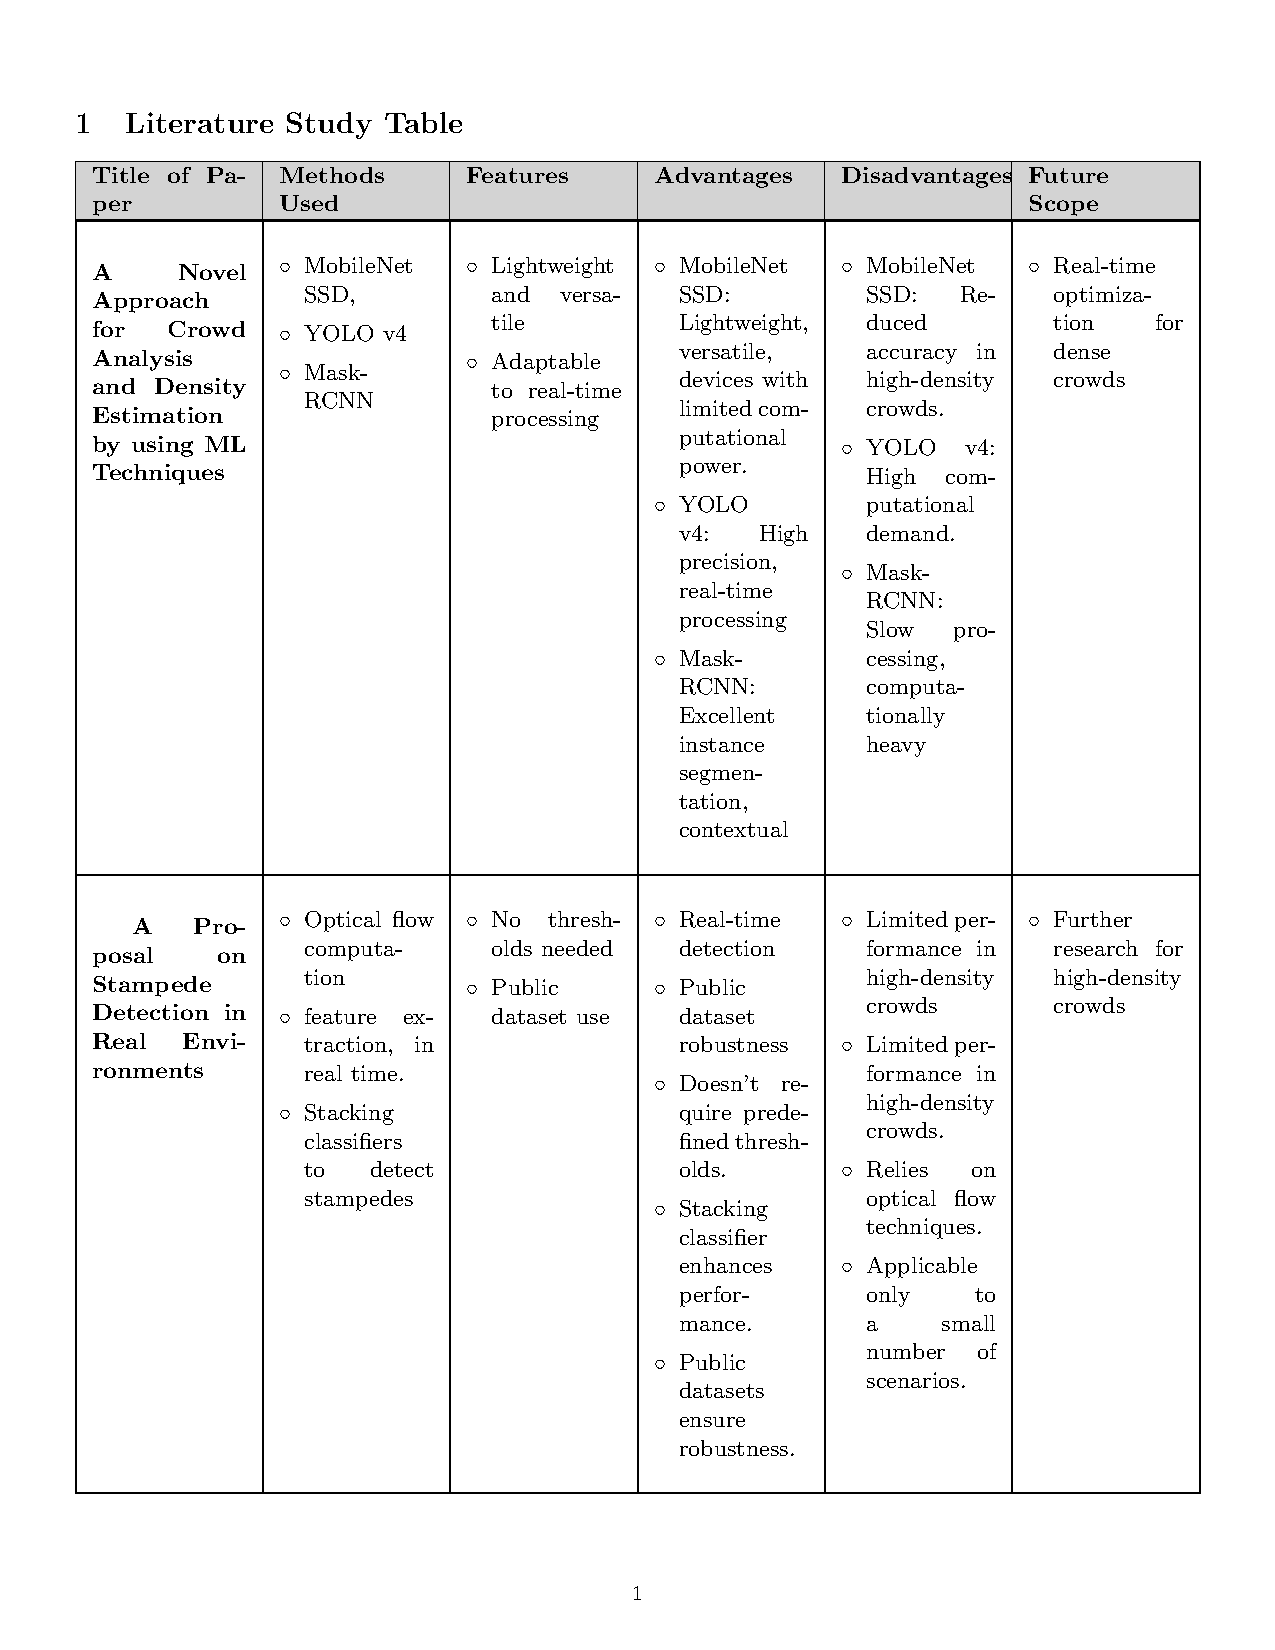
\includepdf[pages=1-4]{LitSurveyTable.pdf}

\section{Literature Survey}
\subsection{Paper 1: A Novel Approach for Crowd Analysis and Density Estimation by using Machine Learning Techniques - V. Kamra, A. Vaishnav, A. Verma, R. Khan, S. Singh}

The paper introduces how Crowd analysis is crucial for urban planning, public safety, and event management. The paper explores the use of the following machine learning algorithms for crowd density estimation: MobileNet SSD, YOLO v4, RCNN. \par
 
\textbf{Methodology : }  
This paper explores the use of MobileNet SSD, YOLO v4, and RCNN for crowd density estimation. These techniques help analyze movement and detect anomalies in crowd behavior. \\

\textbf{Advantages : } 
\begin{itemize}
    \item MobileNet SSD: Lightweight and versatile.
    \item YOLO v4: High precision, suitable for real-time processing. 
    \item RCNN: Excellent for instance segmentation and context handling.
\end{itemize}

\textbf{Disadvantages :}  
\begin{itemize}
    \item MobileNet SSD: Reduced accuracy in high-density crowds.  
    \item YOLO v4: High computational demand.  
    \item RCNN: Slow processing, computationally heavy.
\end{itemize}

\textbf{Inference :}  
This paper provides a foundation for using machine learning techniques for crowd analysis but suggests further optimization for dense crowds. A hybrid model of Mask-R-CNN and YOLO is a probable approach for better stampede prediction systems. We will be implementing this inference in our approach to solving this problem.

\begin{figure}[H]
    \centering
    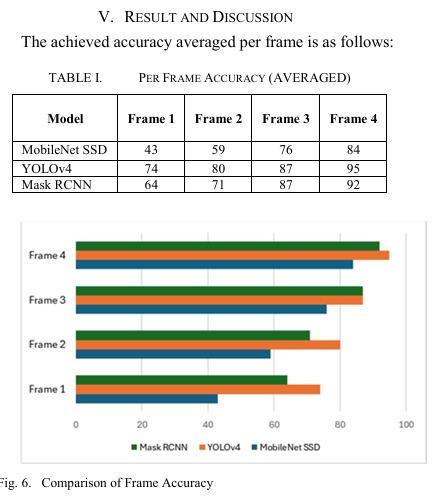
\includegraphics[width=0.75\linewidth]{maskrcnnvscnn.jpg}
    \caption{Comparison of Mask R-CNN, YOLO v4 and MobileNetV2 on crowd density estimation}
\end{figure}

\subsection{Paper 2: A Proposal on Stampede Detection in Real Environments - Antonio Carlos Cob-Parro, Cristina Losada-Gutiérrez, Marta Marrón-Romera, et al.}

This paper presents and approach for real-time stampede detection from images, in low and medium crowd scenarios. The proposal is based on a feature vector extracted from the optical flow entropy, and this does not require the use of thresholds. Instead of that, it includes a a Stacking classifier, based on the union of a random forest with ten estimators and an support vector classifier, that works properly in the different analyzed scenarios. The proposal has been evaluated in UMN and PETS 2009 datasets and compared to other state-of-the-art proposals in terms of accuracy and computational cost.\par
 
\textbf{Methodology :}  
This paper employs optical flow computation, feature extraction, and a stacking classifier to detect stampedes in real time.

\textbf{Advantages :}  
\begin{itemize}
    \item Real-time detection, no need for predefined thresholds.  
    \item Stacking classifier enhances performance.  
    \item Public datasets ensure robustness.
\end{itemize}

\textbf{Disadvantages : }  
\begin{itemize}
    \item Limited performance in high-density crowds.  
    \item Relies on optical flow techniques.
\end{itemize}

\textbf{Inference : }  
While the method performs well in medium-density crowds, further research is required for high-density scenarios.

\begin{comment}
\subsection{Paper 3: Abnormal Crowd Behavior Detection Using Motion Information Images and CNN - Cem Direkoglu}

The paper introduces a method that uses optical flow vectors to generate Motion Information Images (MIIs) for each video frame for detecting abnormal crowd events in surveillance videos, focusing on panic and escape behaviours. MIIs are created by combining optical flow angle differences between consecutive frames and optical flow magnitude. CNN Model is trained on these MIIs to classify normal and abnormal crowd behaviours. The method is evaluated on the UMN and PETS2009 datasets, showing superior performance compared to existing methods. \par

\textbf{Methodology : }  
The method uses optical flow to generate Motion Information Images (MIIs) that are classified using CNN for detecting abnormal behaviors.

\textbf{Advantages}  
\begin{itemize}
    \item MIIs allow for better representation of crowd motion.  
    \item Achieves state-of-the-art results in datasets like UMN and PETS2009.
\end{itemize}

\textbf{Disadvantages}  
\begin{itemize}
    \item Computationally intensive due to optical flow.  
    \item Limited to binary classification (normal/abnormal behavior).
\end{itemize}

\textbf{Inference : }  
The paper demonstrates superior detection of abnormal crowd behaviors but may benefit from multi-class detection.
\end{comment}

\begin{comment}
\subsection{Paper 4: TransCrowd: Weakly-Supervised Crowd Counting with Transformers - Dingkang Liang, Xiwu Chen, Wei Xu, et al.}

 Mainstream crowd counting methods rely on CNNs to regress density maps using point-level annotations, but these are costly and redundant. Weakly-supervised CNN methods with count-level annotations have limited receptive fields, while Transformers provide a global field for better context modelling. This paper proposes the use of TransCrowd, a Transformer-based method for weakly-supervised crowd counting that outperforms CNN-based methods and competes with fully-supervised approaches on five benchmark datasets. \par

\textbf{Methodology : }  
A weakly-supervised Transformer-based model is used for crowd counting, leveraging count-level annotations and global receptive fields.

\textbf{Advantages}  
\begin{itemize}
    \item Transformers offer a global field for better context modeling.  
    \item Works with cheaper count-level annotations.  
\end{itemize}

\textbf{Disadvantages}  
\begin{itemize}
    \item Requires large datasets for training.  
    \item Transformers are more computationally expensive than CNNs.
\end{itemize}

\textbf{Inference : }  
This method outperforms CNN-based methods but needs further validation on diverse datasets.
\end{comment}
\subsection{Paper 3: Background Subtraction in Real Applications: Challenges, Current Models and Future Directions}

Background subtraction is a fundamental technique in computer vision used to distinguish foreground objects from a static or dynamic background. It plays a crucial role in applications such as surveillance, motion detection, and object tracking. This paper explores various methodologies for background subtraction and evaluates their effectiveness in different scenarios.

\textbf{Methodology : }
The paper examines multiple background subtraction algorithms, including Gaussian Mixture Models (GMM), ViBe, and deep learning-based approaches. The key aspects covered are:
\begin{itemize}
    \item 	\textbf{Gaussian Mixture Models (GMM)}: Uses a probabilistic approach to model the background and adapt to changes over time.
    \item 	\textbf{ViBe Algorithm}: A pixel-based technique that maintains a history of background values and updates dynamically.
    \item 	\textbf{Deep Learning Methods}: CNN and RNN-based models that learn complex patterns for improved background-foreground segmentation.
\end{itemize}

\textbf{Advantages : }
\begin{itemize}
    \item GMM provides adaptability to illumination changes and dynamic backgrounds.
    \item ViBe is computationally efficient and robust against sudden background variations.
    \item Deep learning models offer superior accuracy in complex environments with occlusions and dynamic elements.
\end{itemize}

\textbf{Disadvantages : }
\begin{itemize}
    \item GMM can be sensitive to sudden lighting changes and requires parameter tuning.
    \item ViBe may struggle with highly dynamic scenes and complex movements.
    \item Deep learning methods demand significant computational resources and large datasets for training.
\end{itemize}

\textbf{Inference : }
Background subtraction techniques are essential for various real-world applications, but each method has trade-offs in accuracy, computational efficiency, and robustness. While traditional approaches like GMM and ViBe remain effective for many tasks, deep learning-based methods provide enhanced performance in complex scenarios. Future research should focus on optimizing deep learning models for real-time applications with minimal computational overhead.


\subsection{Paper 4: CrowdFormer: An Overlap Patching Vision Transformer}

CrowdFormer introduces an innovative Vision Transformer (ViT) model for crowd analysis, enhancing performance through an overlap patching strategy. This method improves feature representation by maintaining spatial continuity and reducing information loss compared to traditional patch-based ViTs.

\textbf{Methodology :} Unlike standard ViTs that use non-overlapping patches, CrowdFormer applies overlapping patches to retain more spatial information. It leverages a transformer-based architecture to capture long-range dependencies in crowd images by Self-Attention Mechanism. Optimized training techniques ensure improved accuracy without significantly increasing computational costs.

\textbf{Advantages : }
\begin{itemize}
    \item Preserves local and global contextual information.
    \item Improves performance on crowd density estimation and localization tasks.
    \item Reduces information loss from non-overlapping patches.
    \item Enhances accuracy while maintaining efficiency.
\end{itemize}

\textbf{Disadvantages : }
\begin{itemize}
    \item Increased computational complexity compared to traditional non-overlapping patch ViTs.
    \item Potential redundancy due to overlapping patches.
    \item Requires careful hyperparameter tuning for optimal performance.
\end{itemize}

\textbf{Inference : }
CrowdFormer demonstrates the effectiveness of the overlap patching strategy in vision transformers, achieving superior results in crowd analysis. The approach balances performance and efficiency, making it a promising technique for real-world applications in dense scene understanding.

\begin{comment}
\subsection{Paper 4: Machine Learning for Dense Crowd Direction Prediction Using Long Short-Term Memory - Abdullah Alajlan, Alaa Edris, et al.}

The paper proposes an LSTM-based model to predict individual agents' future locations. The model will be tested on both structured crowds and unstructured crowds. The goal is to predict individuals' locations based on their walking behaviours, focusing on their chosen direction and average speed. \par


\textbf{Methodology : }  
An LSTM-based model is used to predict individual trajectories in dense crowds, leveraging the cone of vision concept for influence detection.
\begin{itemize}
    \item Suitable for both structured and unstructured crowds.  
    \item Retains long-term dependencies for more accurate predictions.
\end{itemize}

\textbf{Disadvantages : }  
\begin{itemize}
    \item Computationally expensive, requiring high-quality sequential data.  
\end{itemize} 

\textbf{Inference : }  
The paper introduces a promising method for trajectory prediction, but its complexity demands more real-world testing.
\end{comment}

\subsection{Paper 5: Pyramid Vision Transformer: A Versatile Backbone for Dense Prediction - Wenhai Wang, Enze Xie, Xiang Li, et al.}

Vision Transformers (ViTs) have demonstrated strong performance in computer vision tasks but often lack hierarchical feature representation, leading to high computational demands. This paper introduces Pyramid Vision Transformer (PVT), a novel Transformer backbone that incorporates a hierarchical structure, making it more suitable for dense prediction tasks such as object detection and segmentation. PVT outperforms CNN-based backbones while maintaining efficiency.

\textbf{Methodology : }
The PVT model enhances the ViT architecture by introducing a pyramid structure that progressively reduces the spatial dimensions of feature maps while increasing channel depth. The key innovations include a spatial-reduction attention mechanism to mitigate high memory consumption and multi-stage processing to refine feature representations at different scales. These modifications allow PVT to achieve superior performance on dense prediction tasks while maintaining computational efficiency.

\textbf{Advantages : }  
\begin{itemize}
    \item Incorporates a hierarchical feature representation similar to CNNs.
    \item Reduces memory and computational overhead via spatial-reduction attention.
    \item Improves performance on dense prediction tasks such as segmentation and object detection.
\end{itemize}

\textbf{Disadvantages : }
\begin{itemize}
    \item Requires substantial computational resources compared to traditional CNNs.
    \item Transformer-based models generally need large-scale training datasets for optimal performance.
\end{itemize}

\textbf{Inference : }
Pyramid Vision Transformer bridges the gap between CNNs and ViTs, making it a more effective backbone for dense vision tasks. However, further optimizations are needed to enhance real-time processing capabilities and efficiency in resource-constrained environments.

\subsection{Paper 6: PVT v2: Improved Baselines with Pyramid Vision Transformer - Wenhai Wang, Enze Xie, Xiang Li, et al.}

Mainstream transformer-based architectures for vision tasks have recently demonstrated promising performance, yet they often suffer from high computational costs and limited local feature modeling. This paper proposes PVT v2, an improved variant of the original Pyramid Vision Transformer (PVT v1), which introduces three key modifications: a linear spatial reduction attention (LSRA) layer, an overlapping patch embedding (OPE) scheme, and a convolutional feed-forward network (CFFN). These enhancements aim to reduce the computational complexity from quadratic to linear with respect to spatial dimensions, improve local continuity of the extracted features, and remove the limitations imposed by fixed positional embeddings. As a result, PVT v2 achieves competitive performance on image classification, object detection, and semantic segmentation benchmarks while maintaining efficiency.

\textbf{Methodology :} \\
PVT v2 builds upon the hierarchical structure of PVT v1 by incorporating three orthogonal design improvements. First, the LSRA layer uses average pooling to reduce the spatial resolution before the attention operation, thereby reducing both memory and computation costs. Second, the OPE mechanism replaces non-overlapping patch partitioning with overlapping windows to better capture local continuity in the input images. Third, the CFFN integrates convolutional operations into the feed-forward network, effectively modeling local context without relying on fixed positional encodings. Together, these modifications enable the architecture to process variable-resolution inputs efficiently while maintaining strong global and local feature representations.

\textbf{Advantages : }  
\begin{itemize}
    \item The use of LSRA significantly lowers computational complexity, making the model more efficient.
    \item Overlapping patch embedding enhances the extraction of local features, improving the overall representation.
    \item The convolutional feed-forward network contributes to robust feature learning without fixed positional embeddings.
\end{itemize}

\textbf{Disadvantages : }  
\begin{itemize}
    \item Transformer-based models, including PVT v2, can still be computationally intensive compared to traditional CNNs.
    \item The architecture requires careful hyperparameter tuning and large-scale training data to achieve optimal performance.
\end{itemize}

\textbf{Inference : }
Experimental results indicate that PVT v2 not only outperforms its predecessor on key benchmarks such as ImageNet, COCO, and ADE20K, but also competes favorably with other state-of-the-art transformer models. The improved efficiency and enhanced feature representation suggest that the proposed modifications offer a robust and scalable alternative for various vision tasks. Future work may further explore integration with additional local operations or adaptations to other domains.

\begin{comment}
\subsection{Paper 8: Fusion of CCTV Video and Spatial Information for Automated Crowd Congestion Monitoring - Vivian W. H. Wong, Kincho H. Law}

 Crowd congestion is one of the main causes of modern public safety issues like stampedes. Manual observation using CCTV is error-prone and tedious. The paper proposes a method that combines computer vision and machine learning to enhance crowd safety in public spaces. The framework uses CCTV footage and floor plan information to analyze crowd movement and predict congestion.   This framework uses deep learning-based computer vision models, geometric transformations, and Kalman filter-based tracking algorithms to automate the retrieval of crowd congestion data, specifically the spatio-temporal distribution of individuals and the overall crowd flow. The resulting collective crowd movement data is then stored in the CMGraphs, which are designed to facilitate congestion forecasting at key exit/entry regions. \par
 
\textbf{Methodology : }  
Combines CCTV video and spatial data using crowd mobility graphs for real-time congestion monitoring.

\textbf{Advantages}  
\begin{itemize}
    \item Predictive capabilities and real-time monitoring.  
    \item Effective in visualizing congestion across urban spaces.
\end{itemize}

\textbf{Disadvantages}  
\begin{itemize}
    \item Relies heavily on video quality and computational resources.  
    \item Struggles with dense crowds.
\end{itemize}

\textbf{Inference :}  
This method is efficient for real-time monitoring but needs improvements for higher density crowds.

\end{comment}



\begin{comment}
\subsection{Paper 7: CvT: Introducing Convolutions to Vision Transformers - Haiping Wu, Bin Xiao, Noel Codella, et al.}

Mainstream Vision Transformers (ViTs) lack the inherent inductive biases of Convolutional Neural Networks (CNNs), leading to increased data and computational requirements. This paper introduces Convolutional Vision Transformers (CvT), which incorporate convolutional layers into the ViT framework to enhance locality, reduce computational complexity, and improve feature learning. CvT achieves state-of-the-art performance on multiple image classification benchmarks while maintaining efficiency. \par

\textbf{Methodology: }
The proposed CvT model integrates convolutions into the Transformer architecture by replacing standard self-attention layers with convolutional token embedding and projection mechanisms. This enhances the locality of feature extraction while preserving the global representation power of self-attention. The model also utilizes hierarchical feature representation to reduce computational overhead.

\textbf{Advantages}
\begin{itemize}
    \item Improves feature locality using convolutional embedding.
    \item Reduces computational complexity compared to standard ViTs.
    \item Achieves superior performance on image classification tasks.
\end{itemize}

\textbf{Disadvantages}
\begin{itemize}
    \item Still computationally expensive compared to traditional CNNs.
    \item Requires careful tuning of convolutional and attention components.
\end{itemize}

\textbf{Inference: }
The CvT model bridges the gap between CNNs and ViTs, making Transformers more efficient and effective for computer vision tasks. However, further optimization is needed for real-time applications.
\end{comment}

\subsection{Paper 7: Transformers in Time Series: A Survey}

Transformers have revolutionized various domains of machine learning, particularly in natural language processing (NLP). This paper surveys the application of Transformer models in time series forecasting and analysis, examining their effectiveness compared to traditional and deep learning-based methods. The study highlights the strengths and challenges of using Transformers in time-dependent data modeling.

\textbf{Methodology : }
The survey explores different Transformer architectures adapted for time series analysis. These architectures modify the self-attention mechanism to better capture temporal dependencies while reducing computational complexity. Key techniques include:
\begin{itemize}
    \item 	\textbf{Sparse Attention Mechanisms}: Reducing the quadratic complexity of standard self-attention.
    \item 	\textbf{Positional Encoding Enhancements}: Introducing alternative positional encoding schemes tailored for continuous data.
    \item 	\textbf{Hybrid Models}: Combining Transformers with recurrent or convolutional networks (CNN) to leverage their strengths in sequential data modeling.
    \item 	\textbf{Efficient Training Strategies}: Using windowing and memory-efficient attention mechanisms to scale to long time series.
\end{itemize}

\textbf{Advantages : }
\begin{itemize}
    \item Capable of capturing long-range dependencies in time series data.
    \item Flexible architectures that can be adapted for different forecasting tasks.
    \item Handles multi-modal and irregular time series data more effectively than traditional models.
    \item Advances in sparse attention make Transformers more computationally efficient for time series applications.
\end{itemize}

\textbf{Disadvantages : }
\begin{itemize}
    \item High computational complexity, especially for long sequences.
    \item Requires large-scale training data to generalize well.
    \item Model interpretability remains a challenge compared to traditional statistical methods.
    \item Hyperparameter tuning can be complex and time-consuming.
\end{itemize}

\textbf{Inference : }
Transformers have demonstrated superior performance in various time series applications, but they are not always the best choice for all scenarios. Efficient adaptations are necessary to handle long-term dependencies while keeping computational costs manageable. Future work should focus on improving interpretability, robustness, and efficiency to make Transformers more accessible for real-world time series forecasting.
\subsection{Paper 8: JHU-Crowd++: Large-Scale Crowd Counting Dataset and Benchmark Method - Vishwanath A. Sindagi, Rajeev Yasarla, Vishal M. Patel}

This paper introduces a new large scale unconstrained crowd counting dataset (JHU-CROWD++) that contains “4,372” images with “1.51 million” annotations. In comparison to existing datasets, the proposed dataset is collected under a variety of diverse scenarios and environmental conditions. Specifically, the dataset includes several images with weather-based degradations and illumination variations, making it a very challenging dataset.  \par

\textbf{Methodology : }  
The paper presents a large-scale crowd counting dataset (JHU-CROWD++) and a benchmark method.

\textbf{Advantages : }  
\begin{itemize}
    \item Diverse scenarios and environmental conditions.  
    \item Rich annotations at both image and head level.
\end{itemize}

\textbf{Disadvantages : }  
\begin{itemize}
    \item Complexity of annotations.  
    \item Limited focus on temporal data.
    
\end{itemize}

\textbf{Inference : }  
The paper offers a comprehensive dataset for crowd counting, though further exploration of temporal data is necessary.
\begin{comment}
\subsection{Paper 11: A CNN-RNN Neural Network Join Long Short-Term Memory For Crowd Counting - Jingnan Fu, Hongbo Yang, et al.}

Crowd analysis is crucial for urban planning, public safety, and event management.This report explores the use of machine learning algorithms, CNN-RNN Neural Network Join Long Short-Term Memory for crowd counting and crowd density estimation. \par

\textbf{Methodology : }  
The paper utilizes CNN for feature extraction and LSTM for contextual relevance to estimate crowd density.
    
\textbf{Advantages}  
\begin{itemize}
    \item High accuracy in dense crowds.  
    \item Improved robustness across varying crowd densities.
\end{itemize}

\textbf{Disadvantages}  
\begin{itemize}
    \item Poor performance in sparse crowds.  
    \item High computational complexity.
\end{itemize}

\textbf{Inference : }  
The approach is effective for high-density scenes but needs optimization for sparse environments.
\end{comment}

\chapter{Problem Statement and Solution}
 \section{Problem Statement}
    \subsection{\label{ps}Problem Statement}
    
Stampedes in densely populated areas, such as religious gatherings, concerts, and public events, pose a significant threat to public safety, often leading to severe injuries and fatalities. Traditional crowd monitoring methods rely on manual surveillance or real-time tracking, which can be resource-intensive and prone to human error. How can we develop a robust system that analyzes recorded crowd footage to detect high-risk crowd conditions, assess potential stampede threats, and provide actionable insights to enhance future crowd management and safety measures?

    \subsection{Proposed Solution}
This project develops a Hybrid Model for Stampede Detection and Analysis using Transformers, YOLOv5, and Mask R-CNN for crowd monitoring from recorded video footage. The Transformer model estimates crowd density, while YOLOv5 and Mask R-CNN handle object detection and crowd counting. A discriminator module enhances accuracy by comparing density estimates with actual counts, accounting for environmental factors. \\

By identifying high-risk crowd situations, this system helps authorities implement preventive measures, reducing the likelihood of stampedes. Its impact extends to enhancing public safety at large gatherings, supporting better crowd management, and minimizing casualties in densely populated events.

\subsection{Innovation}
Our Hybrid Model for Stampede Detection and Analysis using Transformers, YOLOv5 and Mask R-CNN introduces a novel approach to crowd monitoring and early warning mechanisms by integrating cutting-edge deep learning techniques. The key innovations in our system include:
\begin{enumerate}
    \item Hybrid Deep Learning Architecture :
    \begin{itemize}
        \item Unlike traditional stampede detection methods that rely solely on optical flow or background subtraction, our system combines Transformers, YOLOv5, and Mask R-CNN for comprehensive crowd analysis.
        \item The Time Series Transformer leverages its ability to capture long-range dependencies and complex temporal patterns in crowd movement data, enhancing the accuracy of crowd analysis and risk assessment.
    \end{itemize}

\item Multi-Model Validation for Enhanced Accuracy
\begin{itemize}
    \item A discriminator module cross-verifies the crowd density estimated by the Transformer model with the object counts from YOLOv5 and Mask R-CNN, ensuring high reliability in dynamic environments.
    \item This hybrid approach mitigates overestimation or underestimation errors common in single-model detection systems.
\end{itemize}
\item Adaptive Background Subtraction for Motion Segmentation 
\begin{itemize}
    \item We incorporate MOG2 background subtraction to enhance motion segmentation, filtering out irrelevant background noise and improving crowd movement anomaly detection.
    \item This allows our system to adapt to different environments, reducing false alarms caused by lighting changes or minor movements.
\end{itemize}
\end{enumerate}


\chapter {Software Requirements Specification}
\section{Introduction}
\subsection{Purpose}
	The purpose of this document is to outline the requirements and functional specifications for a A Hybrid Model for Stampede Detection and Analysis Using YOLOv5, Mask R-CNN, and Time-Series Transformer. This system aims to enhance public safety during large gatherings in India, characterized by high population density and diverse cultural events. By leveraging advanced deep learning techniques, the system will provide  crowd monitoring and early warning mechanisms to detect hazardous crowd conditions, thus preventing potential stampedes and ensuring the safety of attendees.
\subsection{Document Convention}
    This document follows MLA (Modern Language Association) Format. The boldfaced text has been used to emphasize section and sub-section headings. Highlighting is to point out words in the glossary and italicized text is used to label and recognize diagrams. 
    This SRS follows the universally accepted norms used for a formal document. There 
    special conventions used, are listed as follows:
    \begin{itemize}
        \item Bold letters and words signify special importance to those words in that particular context
        \item Words which are in title case or uppercase in the middle on any particular sentence also
        signify the emphasis on those words in the context of the topic
    \end{itemize}
    
    We have also used multiple short forms in this SRS. The most important ones to be noted are
    mentioned as follows:
    \begin{itemize}
        \item CNN: Convolutional Neural Network
        \item RCNN: Region-based Convolutional Neural Network
        \item ML: Machine Learning
        \item DL: Deep Learning
        \item CCTV: Closed-Circuit Television
    \end{itemize}

\subsection{Intended Audience and Reading Suggestions}
This document is used for explaining the functional and non-functional requirements of the project. The document also provides the reader a general understanding about the features and functionalities of the software application and user documentation.
 \newline
 \textbf{Types of Audience}
\begin{itemize}
    \item Developer: The developer who wants to read, change, modify or add new requirements into the existing program may need first to consult this document and update the requirements in an appropriate manner so as not to change the actual purpose of the system or make the system inconsistent.
    \item Event Managers or Local Authorities: who are responsible for ensuring crowd safety and managing large gatherings, as well as making informed decisions based on  local video data of crowd  and swift alerts provided by the application.
\end{itemize}

\subsection{Project Scope}

The scope of the project encompasses the design, development, and implementation of the Crowd Stampede Detection System, including its integration with existing video surveillance infrastructure. The system will be tailored for various public events across India, taking into account the unique challenges posed by high-density crowds and diverse cultural contexts. The project will focus on developing robust algorithms for  crowd monitoring and early warning mechanisms for stampede prediction, and ensuring effective communication channels for alert dissemination. Ultimately, the project aims to contribute to safer public events and minimize the risks associated with large gatherings. 
\subsection{Overview of Developer’s Responsibilities}
The objectives of the proposed system include:

\begin{itemize}
    \item Implementation of advanced algorithms using RCNN and Time-Series Transformer for crowd monitoring and anomaly detection, ensuring accurate predictions of potential stampede situations.
    
    \item Ensuring seamless integration of the Crowd Stampede Detection System with existing video surveillance and monitoring infrastructure for enhanced situational awareness.
    
    \item Conducting thorough testing and validation of the system to ensure reliability and effectiveness in real-world scenarios.
    
    \item Providing comprehensive documentation and training materials for end users, including event managers and local authorities, to facilitate effective utilization of the system.
\end{itemize}

 
\section{Overall Description}
\subsection{Product Perspective}

    Large crowds are a common feature of public events, such as religious gatherings, concerts, and festivals in India. These gatherings often lead to high risks of human-made disasters, particularly stampedes, when overcrowding or sudden panic results in unmanageable surges of movement. The existing monitoring and safety measures are inadequate for predicting and managing these risks, resulting in tragic incidents during large events. 
    \newline
    The challenges of effectively monitoring crowd dynamics and predicting dangerous situations are compounded by the limitations of traditional monitoring systems, which often lack swift response to potential sign of disasters and rely heavily on manual observation. Consequently, there is a critical need for a proactive solution to enhance crowd safety and prevent potential tragedies. The Crowd Stampede Detection System serves as a proactive solution that stakeholders, including event organizers, security personnel, and local authorities, can integrate into their existing crowd management protocols. This system leverages advanced deep learning techniques to enhance situational awareness and provide timely alerts, addressing the critical need for improved crowd safety during public gatherings.

\subsection{Product Functions}
\begin{itemize}
    \item \textbf{Real-Time Crowd Monitoring:} The system analyzes video feeds of at-risk areas to assess crowd density and movement patterns, providing a comprehensive view of the crowd dynamics.
    \item \textbf{Anomaly Detection:} Utilizing RCNN and Transformer algorithms, the system  identifies potential hazards and anomalies in crowd behavior, predicting situations that could lead to stampedes.
    \item \textbf{Alert Notification:} The system generates timely alerts for event organizers and security personnel when dangerous conditions are detected, enabling proactive measures to ensure crowd safety.
    \item \textbf{Historical Data Analysis:} The system stores and analyzes historical crowd data to improve future event planning and risk management strategies.
\end{itemize}

\subsection{User Classes and Characteristics}
\begin{itemize}
    \item \textbf{Event Organizers:} Individuals responsible for planning and managing events who need access to video feed of crowd data and alerts to make informed decisions.
    \item \textbf{Security Personnel:} Staff assigned to maintain safety during events, requiring immediate access to alerts and incident reports to respond effectively to potential risks.
    \item \textbf{System Administrators:} Technicians who maintain the software and hardware components of the Crowd Stampede Detection System, requiring full access to all system functionalities and data management capabilities.
    \item \textbf{Local Authorities:} Government officials responsible for public safety who may need insights into crowd management and incident reports for regulatory and safety compliance.
\end{itemize}

\subsection{Technological Stack}
\begin{itemize}
    \item \textbf{Operating System:} Windows, Linux
    \item \textbf{Programming Languages:} Python
    \item \textbf{Integrated Development Environment (IDE):} Visual Studio Code
    \item \textbf{Deep Learning Frameworks:} PyTorch for building and training machine learning models.
    \item \textbf{High-Level Neural Networks API:} Keras for simplifying the construction of deep learning models.
    \item \textbf{Computer Vision Libraries:} OpenCV, PIL for image and video processing tasks.
    \item \textbf{Frontend Technologies:} React with TypeScript and Tailwind CSS for building a responsive and efficient user interface.
    \item \textbf{Media Processing:} FFmpeg for handling video/audio encoding and decoding tasks and Pillow for image loading and manipulation.
    \item \textbf{Gradio:} Enables an interactive web-based interface for real-time object detection.
\end{itemize}

    \begin{itemize}

        \item \textbf{Version Control System (VCS):} GitHub is used as the version control system for the project. It offers a distributed version control platform that allows for efficient collaboration, code review, and seamless integration with other development tools. GitHub provides features such as branching, merging, pull requests, and issue tracking, enabling effective team collaboration and version control management.
        
        \item \textbf{Package Manager:} pip (Pip Installs Packages) is utilized as the package manager for the project. It is the default package manager for Python applications and provides a comprehensive repository of open-source libraries and packages. pip simplifies the process of installing, managing, and updating project dependencies, ensuring efficient management of external modules used in the crowd stampede detection system.

        \end{itemize}
 \subsection{General Constraints}
        \begin{itemize}
            \item Processing may be affected by low-quality or large video files.
            \item Requires high computational resources for deep learning models.
            \item Handling user video input data requires robust security measures to prevent data breaches.
        \end{itemize}

\subsection{Operating Environment}

    The operational framework of the A Hybrid Model for Stampede Detection and Analysis Using YOLOv5, Mask R-CNN, and Time-Series Transformer is tailored to cater to the distinctive requirements of high-crowd areas such as cultural events, performance shows, concerts etc, ensuring optimal functionality for both users and store owners. The foundational components of the operational environment are outlined below.

\subsection{Design \& Implementation Constraints}
        \begin{itemize}
            \item  Using this system is fairly simple and intuitive. A user familiar with basic application navigation skills should be able to understand all functionality provided by the system.
             \item System shall be able to interface with other components according to their specifications.
            \item The system is limited by its operating server in terms of the maximum number of users it can support at a given time.
            \item Safety and Security Considerations: The system adheres to safety and security policies.
            \item Regulatory Policies: NA
            \item Interfaces to other applications: NA
            \item Parallel operations: NA
            \item Control functions: NA
        \end{itemize}

\subsection{User Documentation}
\begin{itemize}
    \item  User documentation will consist of the several components usually expected of a machine learning and analysis system.
     \item Detailed user’s manual will be provided in a ReadMe file in the GitHub repository.
\end{itemize}

\subsection{Assumptions and Dependencies}
\subsubsection{Assumptions}
\begin{itemize}
    \item The system will have access to a stable and high-speed internet connection for stampede riska analysis via website.
    \item Cameras used for capturing video input will be compatible with the system and positioned to provide optimal coverage of crowd areas.
    \item Event organizers and security personnel will be trained to use the system effectively and respond to alerts generated by the application.
    \item The processing hardware will meet the minimum specifications required for running the deep learning models used in the system.
\end{itemize}

\subsubsection{Dependencies}
\begin{itemize}
    \item The system depends on the availability of high-quality video feeds from cameras to ensure accurate crowd detection and analysis.
    \item The system relies on established deep learning frameworks (e.g., TensorFlow, Keras) for implementing the machine learning algorithms.
    \item Regular maintenance and updates of the software will be necessary to ensure compatibility with evolving hardware and technology standards.
\end{itemize}
        
\section{External Interface Requirement's}
\subsection{User Interfaces}
The system shall offer an intuitive user interface, allowing operators to monitor videos/live video feed, view crowd analysis, and receive alerts on potential stampede situations. The interface will include options to configure thresholds and review logs for past incidents. A dashboard will display key statistics, such as crowd density and warning levels, facilitating quick decision-making.

\subsection{Hardware Interfaces}
\begin{itemize}

    
    \item \textbf{Computational Resources:} Sufficient CPU and GPU resources will be required to run the stampede
    detection model. Hardware should meet the system’s computational needs for processing live video feeds and running deep learning models.
    
    \item \textbf{Data Storage:} Adequate storage will be needed for storing recorded video data, processed results, and historical logs of detected incidents and crowd metrics.
    
    \item \textbf{Deployment Platforms:} The system may be deployed on cloud platforms or local servers, and must be compatible with the chosen environment. The hardware interface should ensure smooth data processing and efficient resource use.

    \item \textbf{Input Devices:} The system should support standard input devices like keyboards, mice, or touchscreens. These will enable the user to interact with the interface to configure settings, upload video streams, and manage alerts. 
\end{itemize}

\subsection{Software Interfaces}
\begin{itemize}
    \item \textbf{Preprocessing Unit:} The video frames from live feeds are provided to this unit for resizing, normalization, and other preprocessing steps. Several preprocessing techniques are applied, including frame extraction and background noise reduction, to prepare the video frames for further analysis by the detection model.

    \item \textbf{Training and Classification:} Several deep learning network architectures, including YOLOv5, Mask R-CNN and Transformers, will be studied. The architecture with the highest efficiency and performance will be selected. By combining object detection with temporal analysis, better performance is achieved in detecting high-density crowd formations and predicting potential stampede risks.

    \item \textbf{Crowd Detection and Analysis Module:} The input video feed will be processed through the detection module, which will use Transformers, YOLOv5 and Mask R-CNN to analyze crowd density and predict potential stampede risks.
    
    \item \textbf{Alert System:} The system will trigger alerts based on detected anomalies in the crowd behavior. Alerts will be communicated through various channels like email or SMS, and displayed on the user interface for immediate action.
    
    \item \textbf{Data Logging and Reporting Module:} This module will record detected incidents and system performance metrics. It will also generate reports for review and audit purposes, which can be exported by the user.
\end{itemize}

\subsection{Communication Interface}
 \textbf{Network Communication:} The system will use standard network protocols (TCP/IP, HTTP) to transmit video data from cameras and send alerts to connected systems or personnel. 

\section{ Hardware \& Software Requirements}
    \subsection{Hardware Requirements}
    \begin{itemize}
        \item Operating System: Windows 8 and above, Linux, macOS
        \item Laptop or Desktop
        \item Camera: Good quality, 3MP
        \item RAM: 8GB or more
        \item Internet Connection: Minimum 100 Mbps bandwidth
        \item Processor: 3GHz Intel i5 or more
        \item Hard Disk: 1TB
\end{itemize}

\subsection{Software Requirements}
Software requirements include:

\begin{itemize}
    \item \textbf{Operating System:} Any operating system (preferably Linux (64-bit), Windows). Linux and Windows are preferred because they are developer-friendly, have a powerful shell, are flexible, and are the most popular.
    
    \item \textbf{Languages:} Python 3. The Python programming language is used for implementing this project as it supports a wide range of libraries for machine learning such as Sci-kit Learn, Pandas, NumPy etc. It has well-written documentation and a large community, which improves development time. It has efficient high-level data structures and a simple but effective approach to object-oriented programming. Python's elegant syntax and dynamic typing, along with its interpreted nature, make it an ideal language for scripting and rapid application development in many areas on most platforms. Python's approach to the object-oriented paradigm makes it easier to divide modules and collaborate on projects. Python's inbuilt functions for reading and writing files allow it to work on multiple file formats and images.
     \item \textbf{IDE:} Google Colab, Visual Studio Code
    \begin{itemize}
        \item \textbf{Google Colaboratory} is a free cloud service by Google that supports free GPU. It provides us with a cloud environment consisting of an n1-highmem-2 instance machine type, 2 virtual CPUs at 2.2GHz, 13GB RAM, and 64GB free space. It has an idle cut-off of 90 minutes and can be used to run code for free for a maximum of 12 hours.
        
        \item \textbf{Visual Studio Code} is a source-code editor developed by Microsoft for Windows, Linux, and macOS. It includes support for debugging, embedded Git control, syntax highlighting, intelligent code completion, snippets, and code refactoring.
    \end{itemize}

        \item \textbf{PyTorch:} A widely used deep learning framework in computer vision, offering dynamic computation graphs and efficient GPU acceleration for tasks like image classification, object detection, and segmentation.
    
        \item \textbf{Keras:} A high-level neural networks API, written in Python and capable of running on top of TensorFlow, Theano, or CNTK. Keras simplifies the process of building deep learning models with its user-friendly, modular, and extensible interface, making it ideal for both beginners and professionals.
        
        \item \textbf{OpenCV}: A library of programming functions mainly aimed at computer vision.
        
        \item \textbf{Pillow}: Enables image loading and manipulation.
         
        \item \textbf{Gradio:} Enables an interactive web-based interface for real-time object detection.

         \item \textbf{ffmpeg:} A free and open-source software suite for handling multimedia data such as audio, video, and other formats. It supports recording, converting, and streaming audio and video in various formats and is widely used for media manipulation in applications.    

         \item \textbf{React:} A JavaScript library for building user interfaces, particularly for single-page applications. It enables the development of dynamic and interactive web applications by utilizing a component-based architecture and a virtual DOM for efficient rendering.

        \item \textbf{TypeScript:} A strongly typed superset of JavaScript that enhances code quality and maintainability. It introduces static typing, interfaces, and advanced tooling support, making it ideal for large-scale web applications.
\end{itemize}

\section{Functional Requirements}
 The system shall process locally stored video input from designated cameras for analysis. It shall perform crowd detection to identify individuals in the video feed. It count the number of individuals detected in a defined area. and extract relevant features from detected objects to facilitate analysis. 
 
The system shall conduct crowd density analysis to assess the concentration of individuals in specific areas and implement crowd anomaly detection to identify unusual behaviors or potential threats. It shall also monitor congestion and trigger alerts when crowd density exceeds safe thresholds. The system shall provide a user-friendly dashboard for event organizers and security personnel to view real-time data and alerts.  

\section{Non-Functional Requirements}
\subsection{Security Requirements}
\begin{itemize}
    \item The system shall implement user authentication to ensure that only authorized personnel can access the system and its functionalities. 
    \item The system shall log user activities and access attempts to provide an audit trail for security purposes.
    \item The system shall comply with relevant data protection regulations to safeguard personal information captured in the video feeds.
\end{itemize}

\subsection{Performance Requirements}
\begin{itemize}
    \item The system should be able to support high load of feed. This statement provides a general sense of reliability when the system is under load. It is important that a substantial number of users be able to access the system at the same time, since many event managers operations occur concurrently. The system should be able to handle all the stress. The system should also be fast in operation
    \item The system shall process video feeds with a minimum frame rate of 20 FPS to ensure smooth analysis and detection.
    \item The system shall support simultaneous monitoring of multiple camera feeds without significant performance degradation.
\end{itemize}

\subsection{Safety Requirements}
\begin{itemize}
    \item The system shall provide alerts to event organizers and security personnel to take preventive action when potential stampede conditions are detected.
    \item The system shall include a fail-safe mechanism to ensure continuous operation, even in the event of a hardware or software failure.
    \item The system shall have a backup data storage solution to prevent data loss during unexpected outages.
    \item The system shall ensure that the deployment of cameras and sensors does not create additional hazards for the crowd, such as tripping hazards or obstruction of emergency exits.
\end{itemize}
\subsection{Software Quality Requirements}
    \begin{itemize}
        \item \textbf{Reliability : }The system should ensure accurate and reliable stapede risk prediction. The platform should have minimal downtime to ensure constant availability for both PC coordinators and students
        \item \textbf{User-Friendly :}The system shall be user-friendly, allowing users to navigate the interface easily without extensive training.
        \item \textbf{Scalability : }The system shall be scalable to accommodate varying crowd sizes and different event types.
        \item \textbf{Portability :} This system will be built for a particular system and may not be portable but results to queries will be portable between many environments.
        \item \textbf{Performance : }The platform should have fast response times, especially during peak usage periods, to provide a smooth experience for users. The AI tool's resume analysis should be efficient, providing quick and accurate results.    
        \item \textbf{Maintainable : }The system shall be designed with maintainability in mind, allowing for easy updates and modifications to algorithms or functionalities.
    \end{itemize}
    
These software quality attributes aim to ensure that the our Stampede detection and analysis is not only functional but also reliable and secure for all end-users.

\chapter{System Design}
\section{System Architecture}

The system utilizes Transformers, YOLOv5 and Mask R-CNN for stampede detection and risk assessment. The stored video output from live camera video feeds, are processed for crowd density estimation and object detection, while a discriminator module ensures accuracy by comparing density estimates with actual counts. The architecture consists of following key modules: video pre-processing for capturing and processing feeds, crowd monitoring for object detection and density estimation, and stampede detection for analyzing behavior and triggering alerts. This ensures high accuracy, quick response times and proactive intervention to prevent crowd disasters. \par
\newpage
\begin{figure}[!h]
  \centering
	\begin{center}
            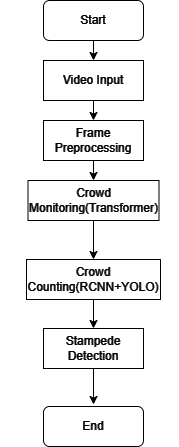
\includegraphics[width=2.85in]{image.png}
        \caption{Outline of the System}
	\end{center}
\end{figure}
\newpage

\section{Use Case Diagram}
\begin{itemize}
    \item \textbf{Description : }
     The system begins by accepting video input from cameras, followed by preprocessing to enhance quality. YOLOv5 and Mask R-CNN detect individuals and perform crowd counting, while a Transformer-based model estimates crowd density. A discriminator module ensures accuracy by comparing density estimates with actual counts. Additionally, a Time-Series Transformer predicts future frame values, enabling anomaly detection by identifying deviations from expected crowd behavior. Real-time alerts are triggered for event organizers and security personnel, ensuring timely intervention and preventing stampedes.
    \item \textbf{Actor :} The actor is the system.
    \item \textbf{Precondition :} The system must be setup in users system.
\end{itemize}

    \begin{figure}[H]
    \centering
	\begin{center}
            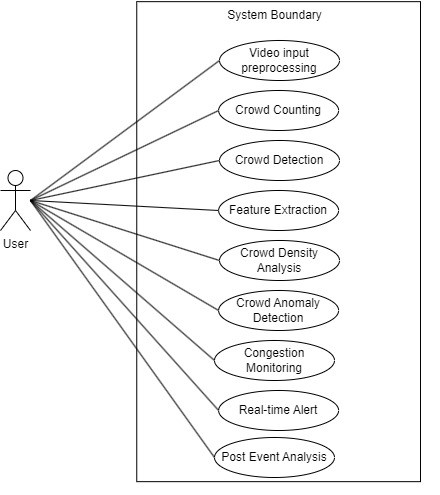
\includegraphics[width=4.8in]{usecasediag.jpg}
        \caption{Use Case Diagram}
        \end{center}
    \end{figure}
\newpage
    
\section{Dataset Design}

We utilise the JHU-CROWD++ Dataset along with frames captured from live video feed. The specifications are as below: 
\begin{itemize}
    \item \textbf{Number of Images:} The dataset consists of a total of 4,372 images.
    \item \textbf{Dimensions:} Images have an average dimension of 910 × 1,430 pixels.
    \item \textbf{Annotations:} There are 1,515,005 head annotations within the dataset, offering rich detail, including:
    \begin{itemize}
        \item \textbf{Head-level/Point-level Annotations:} Each head annotation includes x, y coordinates along with attributes like occlusion level, blur level, and approximate size indicators (width and height).
        \item \textbf{Image-level Annotations:} Annotations at this level provide scene labels (e.g., stadium, rally) and weather conditions (e.g., rain, snow, fog).
    \end{itemize}
    \item \textbf{Dataset Split:} The dataset is divided into two parts:
    \begin{itemize}
        \item \textbf{Part A:} Contains high-density crowd images.
        \item \textbf{Part B:} Contains low-density crowd images.
    \end{itemize}
    \item \textbf{Statistics:} The entire dataset comprises 1,198 images with 330,165 annotations.
    \item \textbf{Additional Large-Scale Dataset:} Recently, Idrees et al. proposed a new large-scale crowd dataset containing 1,535 high-density images with a total of 1.25 million annotations.
    \item \textbf{Diversity:} The dataset features a wide range of images captured under varying conditions, including weather-induced degradations, making it a challenging and comprehensive resource for crowd analysis and detection systems.
    \item \textbf{Frame-by-Frame Dataset Generation:} Since our system captures live camera feeds, the dataset is generated frame-by-frame from the video, enabling detailed and continuous monitoring of crowd dynamics.
\end{itemize}

%%-------- Module Description-------%%%
\section{Module Description}

\subsection{Video Preprocessing Module}
The \textit{Video Preprocessing Module} captures and processes video frames for further analysis. It extracts key frames that highlight significant crowd movements while performing selective frame sampling to reduce redundant data. The selected frames are then undergo noise reduction using Bilateral Filtering to enhance clarity. The module ensures accuracy by preserving temporal dependencies through time-series transformations, maintaining the flow of motion patterns.

\textbf{Tools/Libraries:} OpenCV for video capture and frame extraction, TensorFlow and Keras for preprocessing and normalization, and NumPy for efficient image data handling.

\textbf{Algorithm:}
\begin{itemize}
  \item Step 1: Capture locally stored video in standard formats (e.g., MP4, AVI) using OpenCV.
  \item Step 2: Convert video frames into image frames.
  \item Step 3: Perform selective frame sampling using PyTorch for frame analysis and filtering.
  \item Step 4: Extract key frames using background subtraction method that reflect significant crowd movements or changes.
  %createBackgroundSubtractorMOG2 comes under Gaussian Mixture Models (GMM). It is an implementation of the GMM-based background subtraction method in OpenCV, which models each pixel as a mixture of Gaussians and adapts to dynamic changes in the scene.

  \item Step 5: Apply noise reduction techniques like bilateral filtering for edge preservation.
  \item Step 6: Output preprocessed image frames, ready for further analysis in subsequent modules.
\end{itemize}

\subsection{Crowd Monitoring Module}
The \textit{Crowd Monitoring Module} is responsible for estimating crowd density and counting individuals within each frame. It processes preprocessed image frames using a deep learning model to extract crowd-related features and predict the density of the crowd. The module employs the PVTv2-B5 model to enhance accuracy in feature extraction and density estimation. A frame-wise analysis approach ensures that each frame is independently processed, generating a time-series dataset representing crowd density variations across time. The output includes a crowd density trend graph for visualization and a structured CSV report containing estimated crowd density counts per frame.

\textbf{Tools/Libraries:} PyTorch for Transformer models, OpenCV and Scipy for image processing, Matplotlib  for visualizing crowd density trends over time, NumPy for numerical operations and tensor manipulations, and Pandas for organizing and analyzing data. 

\textbf{Algorithm:}
\begin{itemize}
  \item Step 1: Input preprocessed image frames from the Video Preprocessing Module.
  \item Step 2: Uses PVTv2-B5 to extract relevant crowd features.
  \item Step 3: Predicts crowd density based on extracted features.
  \item Step 4: Ensures non-negative crowd count predictions through ReLU activation.
  \item Step 5: Records estimated crowd count for each frame in CSV format.
  \item Step 6: Plots the crowd density trend over frames for analytical insights.
  \item Step 7: Provides an estimated crowd density count per frame and a density trend graph to aid in decision-making.
\end{itemize}


\subsection{Crowd Counting Module - Part 1}
The \textit{Crowd Counting Module - Part 1} is responsible for detecting and tracking individuals in a crowd using deep learning-based object detection and segmentation techniques. It processes input image frames and identifies people using Mask R-CNN with a ResNet-50 backbone, ensuring accurate localization and counting. The system employs bounding box and mask-based analysis to refine detections, considering only objects with high confidence scores. Additionally, a Gradio-based interactive interface allows users to upload images and receive estimated crowd counts for quick assessments.

\textbf{Tools/Libraries:} PyTorch for running the Mask R-CNN model for object detection, Torchvision for pre-trained models and image processing utilities, and NumPy for numerical computations required for image processing. Pillow for image loading and manipulation.

\textbf{Algorithm:}
\begin{itemize}
  \item Step 1: Input preprocessed frames from the Video Preprocessing Module.
  \item Step 2: Applies Mask R-CNN with a ResNet-50 backbone to detect and localize individuals in each frame.
  \item Step 3: Retains detections with confidence scores above a predefined threshold.
  \item Step 4: Computes the number of detected individuals per frame.
  \item Step 5: Saves detected crowd counts in CSV format for analysis.
  \item Step 6: Provides an object detection report and generates crowd monitoring insights.
\end{itemize}

\subsection{Crowd Counting Module - Part 2}
The \textit{Crowd Counting Module - Part 2} estimates the number of people in a crowd using deep learning-based object detection. It processes preprocessed image frames with YOLOv5, detecting individuals and computing an accurate crowd count. The system implements frame-wise counting, where only detections exceeding a confidence threshold contribute to the final count. 

\textbf{Tools/Libraries:} PyTorch for running the YOLOv5 model for crowd counting, Torchvision for pre-trained models and image processing utilities, OpenCV for handling image and video processing and NumPy for numerical computations required for image processing.

\textbf{Algorithm:}
\begin{itemize}
  \item Step 1: Input preprocessed frames from the Video Preprocessing Module.
  \item Step 2: Uses YOLOv5 for object detection to estimate the number of people in each frame.
  \item Step 3: Counts only individuals detected with a confidence score above a threshold.
  \item Step 4: Plots a crowd density trend graph to analyze variations over time.
  \item Step 5: Saves the estimated crowd count in a CSV file for further analysis.
\end{itemize}

\subsection{Stampede Detection Module}
The \textit{Stampede Detection Module} processes crowd data, including count, positions, movements, and segmentation masks, to track motion and detect potential stampedes. It receives processed frames from the Crowd Monitoring and Counting Modules, where crowd density and count estimates are validated using a discriminator.

\textbf{Discriminator-Based Consistency Check:}

The discriminator compares crowd density estimates from a Transformer-based model with crowd counts obtained from YOLOv5 and Mask R-CNN.

If the crowd count exceeds a predefined threshold, a median fallback mechanism ensures consistency.

\textbf{Transformer-Based Prediction:}

Validated sequential frames are analyzed using a Transformer model to predict future crowd density and count.

The model outputs projected values for upcoming frames, facilitating proactive risk assessment.

\textbf{Stampede Risk Assessment:}

The predicted density and count are fed into a Logistic Regression model to classify stampede risk levels (high or low).

Real-time risk predictions assist in crowd control and emergency response.

\textbf{Tools/Libraries:} PyTorch for building and training the Transformer model to predict crowd density and count, Scikit-Learn utilities for scaling features and training the logistic regression model, NumPy and Pandas.

\textbf{Algorithm:}
\begin{itemize}
  \item Step 1: Input preprocessed image frames with crowd density and crowd count information.
  \item Step 2: A discriminator compares the Transformer-based crowd density estimates with crowd counts from YOLOv5 and Mask R-CNN. If the crowd count exceeds a threshold, a median fallback mechanism is applied.
  \item Step 3: Uses the Transformer model to analyze validated time-series data and predict future crowd density and count.
  \item Step 4: Feeds the predicted crowd density and count into a logistic regression model to classify the risk of a stampede.
  \item Step 5: Displays the predicted crowd density, count, and the assessed risk (high/low) for each future image frame, aiding in efficient crowd monitoring and intervention.
\end{itemize}
%%%%-----------DFD-----------%%%%
\section{Data Flow Diagrams} 

\subsection{Level 0}
\begin{figure}[H]
  \centering
  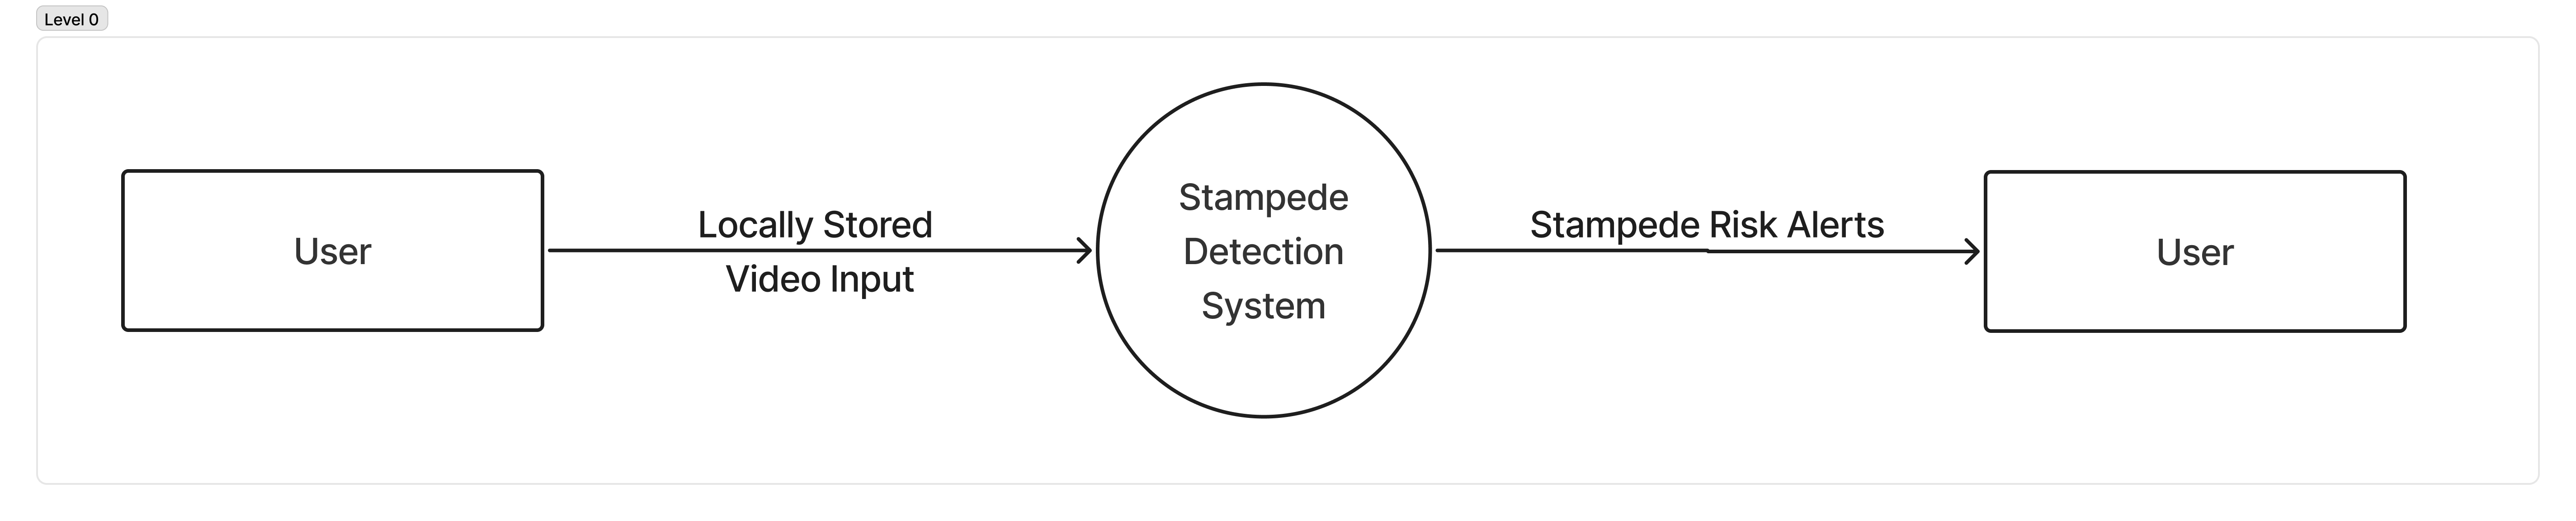
\includegraphics[width=6in]{DFD-0.png}
  \caption{Level 0 Data Flow Diagram}
\end{figure}

\subsection{Level 1}
\begin{figure}[H]
  \centering
  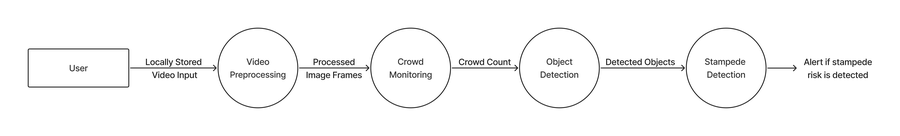
\includegraphics[width=6in]{DFD1.png}
  \caption{Level 1 Data Flow Diagram}
\end{figure}

\subsection{Level 1.1}
\begin{figure}[H]
  \centering
  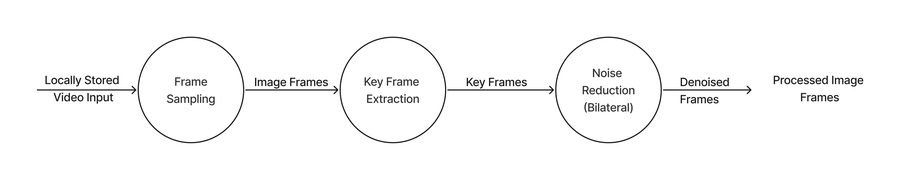
\includegraphics[width=6in]{DFD1.1.png}
  \caption{Level 1.1 Data Flow Diagram}
\end{figure}

\subsection{Level 1.2}
\begin{figure}[H]
  \centering
  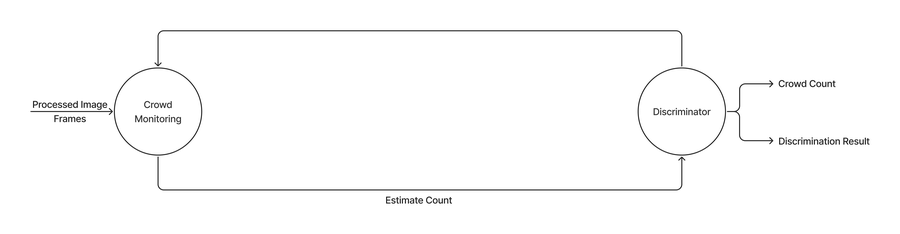
\includegraphics[width=6in]{dfd-cm.png}
  \caption{Level 1.2 Data Flow Diagram}
\end{figure}

\subsection{Level 1.3}
\begin{figure}[H]
  \centering
  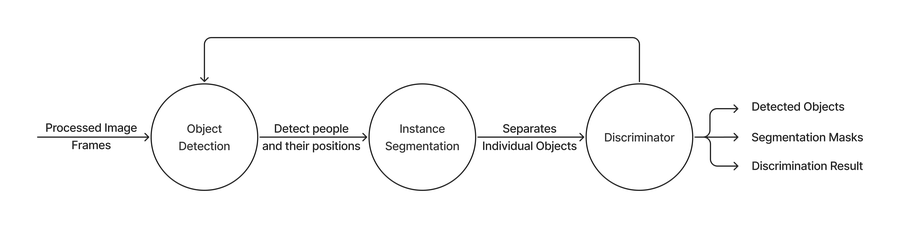
\includegraphics[width=6in]{dfd-od.png}
  \caption{Level 1.3 Data Flow Diagram}
\end{figure}

\begin{comment}
\subsection{Level 1.3 }
\begin{figure}[H]
  \centering
  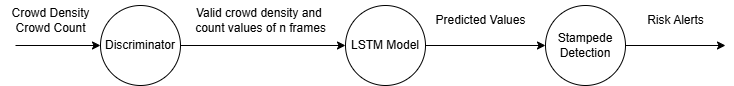
\includegraphics[width=6in]{dfd13.drawio.png}
  \caption{Level 1.3 Data Flow Diagram}
\end{figure}
\end{comment}
\subsection{Level 1.4}
\begin{figure}[H]
  \centering
  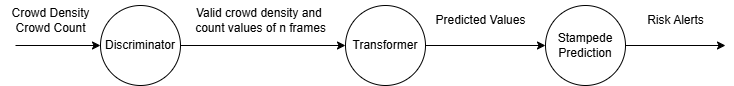
\includegraphics[width=6in]{dfd15.drawio.png}
  \caption{Level 1.4 Data Flow Diagram}
\end{figure}

\begin{comment}
\subsection{Level 1.4 - old}
\begin{figure}[H]
  \centering
  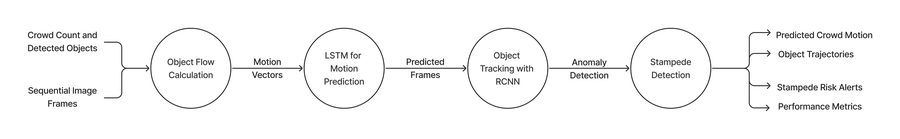
\includegraphics[width=6in]{dfd13.png}
  \caption{Level 1.4 Data Flow Diagram}
\end{figure}
\end{comment}
%%%% --------------- %%%%%

% \chapter{Conclusion}
%  \label {con}
% The project has been successfully implemented, heralding the inception of X - a stampede detection platform


\chapter{Implementation}
\section{Algorithms}
\subsection{Video Preprocessing}
\textbf{Description}
\newline
The algorithm processes video footage by converting it into image frames. To enhance efficiency, selective frame sampling is applied to eliminate redundant data. Key frames, which capture significant crowd movements or changes, are then extracted using background subtraction. These selected frames undergo noise reduction techniques to ensure clarity and consistency. Finally, the preprocessed image frames are structured for further crowd analysis in downstream modules. \\

\textbf{Working of the Algorithm}  
\begin{enumerate} 
    \item \textbf{Accept Input:} Locally stored video in standard formats (e.g., MP4, AVI). 
    \item \textbf{Extract Sample Frames:} Captures video input and converts it into image frames. 
    \item \textbf{Select and Identify Key Frames Using Background Subtraction:} Filters out redundant frames and extracts only those that reflect significant crowd movements or density changes.
    \item \textbf{Reduce Noise:} Applies techniques such as Bilateral blurring to remove unwanted noise and enhance input clarity. 
\end{enumerate}

\textbf{Pseudocode}
%\newline
\begin{algorithm}[H]
    \caption{Capture Video}
\begin{algorithmic}[1]
\Function{CaptureVideo}{$source$}
    \State $cap \gets$ Open video source($source$)
    \If{$cap$ is not opened}
        \State Raise error("Unable to open video source")
    \EndIf
    \State \Return $cap$
\EndFunction
\end{algorithmic}
\end{algorithm}

\begin{algorithm}[H]
\caption{Extract Frames from Video}
\begin{algorithmic}[1]
\Function{ExtractFrames}{$cap$}
    \State $frames \gets []$
    \While{$cap$ has frames}
        \State Read frame from $cap$
        \If{frame is valid}
            \State Append frame to $frames$
        \Else
            \State Break
        \EndIf
    \EndWhile
    \State Release $cap$
    \State SaveIntermediateFrames($frames, "raw\_frames"$)
    \State \Return $frames$
\EndFunction
\end{algorithmic}
\end{algorithm}

\begin{algorithm}[H]
\caption{Sample Frames}
\begin{algorithmic}[1]
\Function{SampleFrames}{$frames, samplingRate$}
    \State $sampledFrames \gets$ Select every $samplingRate$-th frame
    \State SaveIntermediateFrames($sampledFrames, "sampled\_frames"$)
    \State \Return $sampledFrames$
\EndFunction
\end{algorithmic}
\end{algorithm}

\begin{algorithm}[H]
\caption{Extract Key Frames Using Background Subtraction}
% createBackgroundSubtractorMOG2 comes under Gaussian Mixture Models (GMM). It is an implementation of the GMM-based background subtraction method in OpenCV, which models each pixel as a mixture of Gaussians and adapts to dynamic changes in the scene.


\begin{algorithmic}[1]
\Function{ExtractKeyFrames}{$frames$}
    \State $bgSubtractor \gets$ Create background subtractor model
 %   createBackgroundSubtractorMOG2 comes under Gaussian Mixture Models (GMM). It is an implementation of the GMM-based background subtraction method in OpenCV, which models each pixel as a mixture of Gaussians and adapts to dynamic changes in the scene.


    \State Compute initial motion area from first 10 frames
    \State Compute threshold as $averageMotion * 0.005$
    \State $keyFrames \gets [frames[0]]$
    \State $prevMotionArea \gets$ Process($frames[0]$)
    \For{$i = 1$ to $|frames| - 1$}
        \State $currMotionArea \gets$ Process($frames[i]$)
        \If{$|currMotionArea - prevMotionArea| > threshold$}
            \State Append $frames[i]$ to $keyFrames$
        \EndIf
        \State $prevMotionArea \gets currMotionArea$
    \EndFor
    \State SaveIntermediateFrames($keyFrames, "key\_frames"$)
    \State \Return $keyFrames$
\EndFunction
\end{algorithmic}
\end{algorithm}

\begin{comment}
\begin{algorithm}[H]
\caption{Resize Frames}
\begin{algorithmic}[1]
\Function{ResizeFrames}{$frames, size$}
    \State $resizedFrames \gets []$
    \For{each $frame \in frames$}
        \State $resizedFrame \gets$ Resize($frame, size$)
        \State Append $resizedFrame$ to $resizedFrames$
    \EndFor
    \State SaveIntermediateFrames($resizedFrames, "resized\_frames"$)
    \State \Return $resizedFrames$
\EndFunction
\end{algorithmic}
\end{algorithm}
\end{comment}

\begin{algorithm}[H]
\caption{Reduce Noise in Frames}
\begin{algorithmic}[1]
\Function{ReduceNoise}{$frames, method$}
    \State Apply Bilateral filter to each frame
    \State SaveIntermediateFrames($frames, "denoised\_frames"$)
    \State \Return $frames$
\EndFunction
\end{algorithmic}
\end{algorithm}

\begin{comment}
\begin{algorithm}[H]
\caption{Apply Skip Connections to Frames}
\begin{algorithmic}[1]
\Function{ApplySkipConnections}{$frames$}
    \State $model \gets$ Initialize SkipConnections model
    \State $processedFrames \gets []$
    \For{each $frame \in frames$}
        \State $tensorFrame \gets$ Convert frame to tensor
        \State $processedFrame \gets$ Pass $tensorFrame$ through model
        \State Append $processedFrame$ to $processedFrames$
    \EndFor
    \State SaveIntermediateFrames($processedFrames, "skip\_frames"$)
    \State \Return $processedFrames$
\EndFunction
\end{algorithmic}
\end{algorithm}
\end{comment}

\begin{algorithm}[H]
\caption{Save Intermediate Frames}
\begin{algorithmic}[1]
\Function{SaveIntermediateFrames}{$frames, outputDir$}
    \For{$i = 0$ to $|frames| - 1$}
        \State Save frame $frames[i]$ as an image in $outputDir$
    \EndFor
\EndFunction
\end{algorithmic}
\end{algorithm}

\subsection{Crowd Density Prediction using Transformers}
\textbf{Description}  

This algorithm predicts crowd density from preprocessed video frames using a pretrained Transformer-based model. The model takes sequential frames as input, extracts features, and estimates the number of people present in each frame. The predictions are saved for further analysis, such as trend visualization and risk assessment.  

\textbf{Working of the Algorithm}  

\begin{enumerate}
    \item \textbf{Load the Pretrained Model} – The algorithm initializes a Transformer-based model (\texttt{pvt\_v2\_b5}) and loads pretrained weights.  
    \item \textbf{Load Preprocessed Frames} – The preprocessed frames are retrieved from storage, ensuring they are sorted sequentially.  
    \item \textbf{Predict Crowd Counts} – Each frame is processed using the model to extract crowd features and estimate the total count. Activation functions like ReLU are applied to ensure non-negative outputs.  
    \item \textbf{Save the Results} – The predicted crowd density values are stored in a CSV file for further evaluation.  
    \item \textbf{Visualize Trends} – The predicted counts are plotted over time, helping analyze crowd fluctuations.  
\end{enumerate}  

\textbf{Pseudocode}  

\begin{algorithm}[H]
\caption{Load Pretrained Model}
\begin{algorithmic}[1]
\Function{LoadPretrainedModel}{$weightsPath$}
    \State $device \gets$ Set computation device to CPU
    \State $model \gets$ Initialize \texttt{pvt\_v2\_b5} model
    \State $weights \gets$ Load weights from $weightsPath$
    \State $model \gets$ Load state dictionary with $weights$
    \State \Return $model$
\EndFunction
\end{algorithmic}
\end{algorithm}

\begin{algorithm}[H]
\caption{Load Preprocessed Frames}
\begin{algorithmic}[1]
\Function{LoadPreprocessedFrames}{$source$}
    \State $frameFiles \gets$ List all .pt files in $source$
    \State Sort $frameFiles$ to maintain sequence
    \State \Return $frameFiles$
\EndFunction
\end{algorithmic}
\end{algorithm}

\begin{algorithm}[H]
\caption{Predict Crowd Counts}
\begin{algorithmic}[1]
\Function{PredictCrowdCounts}{$frames, model$}
    \State $counts \gets []$
    \For{$i = 0$ to $|frames| - 1$}
        \State $frameTensor \gets$ Load tensor from $frames[i]$
        \State $frameTensor \gets$ Add batch dimension
        \State $pred \gets$ model.get\_all\_feats($frameTensor$)
        \State $pred \gets$ Apply ReLU to remove negatives
        \State $count \gets$ Sum all values in $pred$
        \State Append $count$ to $counts$
    \EndFor
    \State \Return $counts$
\EndFunction
\end{algorithmic}
\end{algorithm}

\begin{algorithm}[H]
\caption{Save Crowd Density Data}
\begin{algorithmic}[1]
\Function{SaveCrowdData}{$counts, outputFile$}
    \State Convert $counts$ to CSV format
    \State Save $counts$ as CSV file in $outputFile$
\EndFunction
\end{algorithmic}
\end{algorithm}

\begin{algorithm}[H]
\caption{Plot Crowd Density Trends}
\begin{algorithmic}[1]
\Function{PlotCrowdTrends}{$counts, outputFile$}
    \State Create a plot with $frameNumbers$ on X-axis and $counts$ on Y-axis
    \State Use blue color and markers for visualization
    \State Save plot as $outputFile$
\EndFunction
\end{algorithmic}
\end{algorithm}

\subsection{Crowd Counting using Deep Learning Techniques}

\textbf{Description}  

This algorithm estimates the number of people in an image or video frame using deep learning-based object detection techniques. Models like Mask R-CNN and YOLOv5 are used to detect individuals and count them. Non-Maximum Suppression (NMS) is applied to filter redundant detections, ensuring accurate counting. The final count is displayed and can be integrated into real-time monitoring systems.

\textbf{Working of the Algorithm}  

\begin{enumerate}
    \item \textbf{Load the Pretrained Model} – A deep learning model such as Mask R-CNN or YOLOv5 is loaded with pretrained weights and set to evaluation mode.
    \item \textbf{Load the Input Source} – The input is loaded, which can be an image, a video file, or a real-time stream from a webcam.
    \item \textbf{Perform Inference} – The model processes the image and generates raw predictions, including bounding boxes, class labels, and confidence scores.
    \item \textbf{Apply Non-Maximum Suppression (NMS)} – This step filters overlapping detections, keeping only the most confident bounding boxes for each detected person.
    \item \textbf{Count the People} – Detections classified as "person" and above a confidence threshold are counted.
    \item \textbf{Display the Result} – The final count is displayed on the screen or saved for further analysis.
\end{enumerate}  

\textbf{Pseudocode}  

\begin{algorithm}[H]
\caption{Load Pretrained Model}
\begin{algorithmic}[1]
\Function{LoadPretrainedModel}{$weights$}
    \State $device \gets$ Select computation device (CPU/GPU)
    \State Load YOLOv5 model with given $weights$ on $device$
    \State Set model to evaluation mode
    \State \Return $model$
\EndFunction
\end{algorithmic}
\end{algorithm}

\begin{algorithm}[H]
\caption{Load Input Source}
\begin{algorithmic}[1]
\Function{LoadSource}{$source, imgSize, stride$}
    \If{$source$ is a webcam, video stream, or URL}
        \State Enable CUDA benchmarking for performance
        \State Load real-time or locally stored video stream
    \Else
        \State Load images from given $source$
    \EndIf
    \State \Return $dataset$
\EndFunction
\end{algorithmic}
\end{algorithm}

\begin{algorithm}[H]
\caption{Perform Inference}
\begin{algorithmic}[1]
\Function{PerformInference}{$image, model$}
    \State Run forward pass of $image$ through $model$
    \State \Return $rawPredictions$
\EndFunction
\end{algorithmic}
\end{algorithm}

\begin{algorithm}[H]
\caption{Apply Non-Max Suppression}
\begin{algorithmic}[1]
\Function{ApplyNMS}{$rawPredictions, confThres, iouThres$}
    \State Filter predictions based on confidence threshold $confThres$
    \State Apply Non-Max Suppression (NMS) with IoU threshold $iouThres$
    \State Extract bounding boxes and confidence scores
    \State \Return $filteredPredictions$
\EndFunction
\end{algorithmic}
\end{algorithm}

\begin{algorithm}[H]
\caption{Count People}
\begin{algorithmic}[1]
\Function{CountPeople}{$filteredPredictions$}
    \State Define minimum confidence threshold for detection
    \State Select detections where class = "person" and confidence $\geq$ threshold
    \State $count \gets$ Total number of selected detections
    \State \Return $count$
\EndFunction
\end{algorithmic}
\end{algorithm}

\begin{algorithm}[H]
\caption{Display Crowd Count}
\begin{algorithmic}[1]
\Function{DisplayCount}{$count$}
    \State Show output: "Estimated crowd count: $count$"
\EndFunction
\end{algorithmic}
\end{algorithm}


\subsection{Future Frame Value Prediction using Transformers}

\textbf{Description}  

This algorithm predicts future crowd density and count values from previously observed frames using a Transformer-based deep learning model. The model takes validated crowd features as input, forecasts the crowd distribution for upcoming frames, and assesses potential risk factors for crowd instability. The predictions can be used for proactive risk management and  crowd monitoring.

\textbf{Working of the Algorithm}  

\begin{enumerate}
    \item \textbf{Load the Pretrained Model} – A Transformer-based model is initialized and loaded with pretrained weights for crowd forecasting.
    \item \textbf{Validate and Preprocess Input Data} – The crowd density and count estimates undergo consistency checks using a discriminator. If discrepancies exceed a threshold, the values are adjusted.
    \item \textbf{Predict Future Crowd Values} – The validated input features are processed through the Transformer model to generate forecasts for future crowd density and count.
    \item \textbf{Assess Stampede Risk} – The predicted crowd values are passed to a logistic regression model that estimates the risk of a stampede occurring.
    \item \textbf{Display the Risk Level} – The stampede risk level is displayed, providing early warnings when the probability exceeds a critical threshold.
\end{enumerate}  

\textbf{Pseudocode}  

\begin{algorithm}[H]
\caption{Load Pretrained Model}
\begin{algorithmic}[1]
\Function{LoadPretrainedModel}{$weights$}
    \State $device \gets$ Select computation device (CPU/GPU)
    \State Load Transformer-based crowd forecasting model with given $weights$
    \State Set model to evaluation mode
    \State \Return $model$
\EndFunction
\end{algorithmic}
\end{algorithm}

\begin{algorithm}[H]
\caption{Validate and Preprocess Input Data}
\begin{algorithmic}[1]
\Function{GetValidatedCrowdFeatures}{$crowdDensity, crowdCount$}
    \State Compute consistency check using a discriminator
    \If{$|crowdDensity - crowdCount| > \text{threshold}$}
        \State Apply median fallback to refine crowd count
    \EndIf
    \State Normalize the refined features
    \State \Return validated crowd features
\EndFunction
\end{algorithmic}
\end{algorithm}

\begin{algorithm}[H]
\caption{Predict Future Crowd Values}
\begin{algorithmic}[1]
\Function{PredictFutureCrowdValues}{$input, model$}
    \State Pass validated $input$ through the Transformer model
    \State Predict future crowd density and count values
    \State \Return $predictedDensity, predictedCount$
\EndFunction
\end{algorithmic}
\end{algorithm}

\begin{algorithm}[H]
\caption{Assess Stampede Risk}
\begin{algorithmic}[1]
\Function{PredictStampedeRisk}{$predictedDensity, predictedCount, model$}
    \State Combine the predicted crowd density and count values
    \State Pass combined features through the logistic regression model
    \State \Return $stampedeRisk$
\EndFunction
\end{algorithmic}
\end{algorithm}

\begin{algorithm}[H]
\caption{Display Stampede Risk}
\begin{algorithmic}[1]
\Function{DisplayRisk}{$stampedeRisk$}
    \If{$stampedeRisk > 0.5$}
        \State Show output: "Warning: High risk of stampede!"
    \Else
        \State Show output: "Low risk: No stampede expected"
    \EndIf
\EndFunction
\end{algorithmic}
\end{algorithm}

\section {Implementation - Models used}

The stampede detection system utilizes a combination of deep learning and machine learning models to analyze crowd movement, detect high-risk scenarios, and classify the risk levels of a potential stampede. The core models include:
\begin{enumerate}
    \item YOLOv5 (You Only Look Once Version 5): Used for real-time object detection, specifically identifying individuals in a crowd. It provides bounding box predictions that help in assessing crowd density.
    \item Mask R-CNN (Mask Region-Based Convolutional Neural Network): Performs instance segmentation, allowing precise identification of individual people and their spatial distribution in the crowd. It helps refine crowd density estimates by detecting overlapping individuals.
    \item Vision Transformer (ViT): Enhances crowd segmentation and motion analysis, leveraging self-attention mechanisms to extract spatial and temporal features from video frames.
    \item Logistic Regression Classifier: Takes aggregated data from the YOLOv5 and ViT modules to classify risk levels based on predefined thresholds.
    \item Discriminator Module: Compares outputs from YOLOv5 and ViT to validate accuracy and ensure precise crowd density estimation.
    \item Contrast Enhancement Preprocessing: Used to improve detection performance in low-light environments, ensuring stable performance in varying lighting conditions.
\end{enumerate}

\section {Implementation - Dataset}

The system has been trained and validated using multiple datasets to ensure robustness across different crowd scenarios. The primary datasets include:
\begin{enumerate}
    \item JHU-CROWD++: A large-scale dataset consisting of dense crowd images, providing high-accuracy annotations for crowd counting and density estimation. This dataset is crucial for training the crowd control module and improving the model’s ability to differentiate between normal and high-risk crowd behavior.
    \item ShanghaiTech Dataset: Contains Part A (dense crowds) and Part B (sparser crowds), allowing the model to learn crowd behavior across different scenarios.
\end{enumerate}

\section{Development Tools}
This project utilizes various development tools for model training, evaluation, deployment, and collaboration. Below are some of the key tools used:

\begin{enumerate}
    \item Git \& GitHub : Git is a version control system that helps track code changes, while GitHub is a cloud-based platform for managing repositories. They enable seamless collaboration, version control, and integration with CI/CD pipelines for model deployment and continuous improvement.
    \item Google Colab: Google Colab provides a cloud-based Jupyter Notebook environment that allows for easy execution of deep learning models without requiring local GPU resources. It supports free GPU and TPU acceleration, making it ideal for training transformer-based crowd forecasting models and conducting experiments with large datasets.
    \item Python \& Jupyter Notebook : Python is the primary programming language used for model development. Jupyter Notebook allows interactive coding, making it easier to test and analyze deep learning models, visualize results, and document findings.
    \item PyTorch : PyTorch is an open-source deep learning framework used for developing and training the transformer-based crowd forecasting model. It provides efficient tensor computation, dynamic computation graphs, and support for GPU acceleration.
    \item OpenCV : OpenCV is used for image and video processing, including extracting frames, pre-processing input data, and applying transformations to enhance feature detection for crowd density estimation.
    \item Scikit-learn : Scikit-learn provides essential machine learning tools, including logistic regression, which is used for stampede risk assessment based on predicted crowd density and movement patterns.
    \item Pandas \& NumPy : Pandas and NumPy are used for handling large datasets, performing numerical operations, and pre-processing data for feeding into deep learning models.
    \item Matplotlib \& Seaborn : These visualization libraries help in analyzing crowd patterns, model predictions, and risk assessment outputs by plotting graphs and heatmaps.
    \item \textbf{React:} A JavaScript library for building user interfaces, particularly for single-page applications. It enables the development of dynamic and interactive web applications by utilizing a component-based architecture and a virtual DOM for efficient rendering.
\end{enumerate}

\chapter{Testing}

\section{Testing Methodology}
Software Testing Methodology is defined as strategies and testing types used to certify that the Application Under Test meets user expectations. Test methodologies include functional and non-functional testing to validate the Application Under Test. Each testing methodology has a defined test objective, test strategy, and deliverable. Software testing methodology ensures that software products and systems have been successfully tested to meet their specified requirements and can operate in all anticipated environments with the required usability and security.

Software testing methods are traditionally divided into white-box testing and black-box testing. These two approaches describe the point of view that a test engineer takes when designing test cases. \\

White-box testing examines internal structures or workings of a program, as opposed to testing only the functionality exposed to the end-user. In this method, an internal perspective of the system and programming skills are used to design test cases. The tester chooses inputs to exercise paths through the code and determines the appropriate outputs. White-box testing can be applied at the unit, integration, and system levels of software testing, but it is usually performed at the unit level. \\

Black-box testing treats the software as a black-box, evaluating its functionality without any knowledge of the internal implementation. Testers focus only on what the software is supposed to do, not on how it does it. Black-box testing is applied at the system level in this project. \\

The testing methods applied to the system are as follows:

\begin{enumerate}
    \item Unit Testing: A software development process in which the smallest testable parts of an application, called units, are individually tested to verify their correct operation.

    \item Integration Testing: Conducted after unit testing, where individual software modules are combined and tested as a group.

    \item System Testing: Performed on a complete, integrated system to evaluate its compliance with specific requirements. This type of testing falls within black-box testing, meaning it does not require knowledge of the internal design or logic of the system.
    
    \item Performance Testing : Assesses the system’s efficiency in terms of processing speed, detection accuracy, and response time under different conditions.
\end{enumerate}
\section{Unit Testing}
The following table summarizes the test cases executed at this stage:
\begin{table}[H]
    \centering
    \renewcommand{\arraystretch}{1.4}
    \setlength{\tabcolsep}{3pt}
    \footnotesize
    \begin{tabular}{| m{2.3cm} | m{3.2cm} | m{3.5cm} | m{3.2cm} | m{1.2cm} |}
        \hline
        \textbf{Test Title} & \textbf{Test Condition} & \textbf{System Behavior} & \textbf{Expected Result} & \textbf{Test Status} \\ 
         \hline
         Video Frame Extraction & Input local video file & Frames are extracted correctly & Frames match the input video & PASS \\
        \hline 
        Noise Reduction & Image Frame with sufficient noise & Bilateral filtering removes noise & Clearer output frame obtained & PASS \\
        \hline
        Key Frame Selection & Input video with crowd movement & Key frames are selected	& Only significant movement frames & PASS \\
        \hline
        Crowd Counting (YOLOv5) &	Provide an image with multiple people & YOLOv5 detects and counts people & Count is close to actual number & PASS \\
        \hline 
        Crowd Counting (Mask R-CNN) &	Provide a video with crowded scenes	& Mask R-CNN detects and counts people & Count is close to actual number & PASS \\
        \hline
        Background Subtraction& Provide a video with changing lighting & MOG2 removes background artifacts &	Moving people detected correctly	& PASS \\
        \hline
         Stampede Alert Mechanism  & Simulate/Input Crowd Video & Alert is generated within 2 seconds & Immediate alert is sent & PASS \\ \hline
    \end{tabular}
    \caption{Unit Testing Results}
\end{table}

\section{Integration Testing}
The following test cases were executed:
\begin{table}[H]
    \centering
    \renewcommand{\arraystretch}{1.4}
    \setlength{\tabcolsep}{3pt}
    \footnotesize
    \begin{tabular}{| m{2.3cm} | m{3.2cm} | m{3.5cm} | m{3.2cm} | m{1.2cm} |}
        \hline
        \textbf{Test Title} & \textbf{Test Condition} & \textbf{System Behavior} & \textbf{Expected Result} & \textbf{Test Status} \\ 
        \hline
        Fast Alert Generation &	Simulate high-risk crowd event & System issues alert	& Alert triggered in expected time	& PASS \\
        \hline
        Integration of Modules &  Run full pipeline from frame extraction to alert	& Modules function together without error & Correct results produced & PASS \\
        \hline
        Data Storage \& Reporting &	Run system and check generated logs & System logs density, counts, and alerts	& CSV contains accurate structured data	& PASS \\
        \hline
    \end{tabular}
    \caption{Integration Testing Results}
\end{table}

\section{System Testing}
The test cases include:
\begin{table}[H]
    \centering
    \renewcommand{\arraystretch}{1.4}
    \setlength{\tabcolsep}{3pt}
    \footnotesize
    \begin{tabular}{| m{2.3cm} | m{3.2cm} | m{3.5cm} | m{3.2cm} | m{1.2cm} |}
        \hline
        \textbf{Test Title} & \textbf{Test Condition} & \textbf{System Behavior} & \textbf{Expected Result} & \textbf{Test Status} \\ 
        \hline
         Stampede Detection (High Risk)	& Input video w/ rapid crowd movement &	Model predicts high risk	& Stampede warning is triggered & PASS\\
         \hline
        Stampede Detection (Low Risk) & Input video with normal crowd movement	& Model predicts low risk	& No warning issued	& PASS\\ 
        \hline
        Crowd Density Estimation & Video with varying crowd densities	& Transformer estimates crowd density	& Estimate aligns with real crowd	& PASS\\
        \hline
        Discriminator Accuracy & Compare YOLOv5 \& Transformer estimates & Cross-verifies results & Difference within set threshold	& PASS\\
        \hline 
%        Logistic Regression Classification & Provide test data for risk classification& Logistic regression classifies risk level& Matches expected classification & 	PASS \\
        Low Light Environment & Input video with dim lighting conditions	& Model enhances contrast \& detects people correctly	& Detection accuracy remains high & PASS \\
        \hline
 
        Performance Under Load & System should handle multiple classification requests. & Response time should remain within acceptable limits. & The system classifies images within 3s under load. & PASS \\ 
        \hline
    
    
    \end{tabular}
    \caption{System Testing Results}
\end{table}

\section{Performance Testing}
 Performance testing was conducted to evaluate system efficiency under different conditions:
 
 \begin{itemize}
     \item Accuracy Testing: Measured detection accuracy in various lighting and environmental conditions, achieving an accuracy rate of 89%.
     \item Robustness : The system exhibited Robust behaviour across various environmental conditions and lighting settings (unless extreme variations).
 \end{itemize}

\section{Conclusion}
The A Hybrid Model for Stampede Detection and Analysis Using YOLOv5, Mask R-CNN, and Time-Series Transformer has passed all key tests, ensuring that individual modules, integrated components, and the full system function correctly. The final accuracy achieved in classification is 89\%, demonstrating strong model performance.

\chapter{Graphical User Interface}
The graphical user interface is a user interface that allows users to interact with electronic devices through graphical icons and visual indicators such as secondary notations, instead of text-based user interfaces, typed command labels or text navigation.GUIs were introduced in reaction to the perceived steep learning curve of command-interfaces which require a command to be typed on a computer keyboard. \\

Designing the visual composition and temporal behaviour of a GUI is an important part of software application programming in the area of human-computer interaction. Its goal is to enhance the efficiency and use case for the underlying logical design of a stored program, a designed discipline name usability. Methods for user-centred design are used to ensure that the visual language introduced in the design is well-tailored to the tasks. For several decades GUIs were controlled exclusively by a mouse and keyboard. While these types of input devices are sufficient for desktop computers, they do not work as well for mobile devices, such as smartphones and tablets. Therefore, mobile operating systems are designed to use a touchscreen. Many mobile devices can now be controlled by spoken commands as well. 

\section{GUI Overview}
A GUI uses a combination of technologies and devices to provide a platform that users can interact with, for the task of gathering and producing information. Traditionally, browsers acted themselves as independent and isolated software. All the features that were necessary for the browsers to perform, were implemented in browsers itself. Limitation of this method was that the users had no control over the performance of the browser, or at least they could not do anything to improve its performance. \\

Nowadays, browser performance can be improved by users, especially as the user demands. Users can either develop or get modules such as apps, extensions, plug-ins which can work within the browser. These modules are usually optional and can be installed to improve the user experience of the browser. These modules perform a specific task, which it is designed to do when the user asks to. For instance, there are browser apps which help to give users some reminder, browser extensions which can fill forms automatically, plugins which improve the visual effect of the browser. \\

The website’s GUI is built using modern web technologies, primarily React and Typescript for the frontend, with a responsive design that ensures accessibility across desktops, tablets, and mobile devices. The design principles include clean layouts, visually distinct buttons, and smooth navigation, making the platform efficient and easy to use. 

\section{Main GUI Components}
The main GUI components are:

\begin{enumerate}
    \item \textbf{Landing page:} This page is the home page which mentions the details about the platform such as it’s features and benefits.
    \item \textbf{About Page:} This page provides an overview of the platform, its purpose, and how it helps in stampede detection. It includes details about the technology used, the social impact \& motivation behind the project, and its potential impact.
    \item \textbf{Upload Page:} This page allows users to upload video footage or images for stampede detection analysis. It provides an intuitive interface for selecting files, submitting them for processing, and viewing results.
\end{enumerate}
\begin{itemize}
    \item \textbf{Landing Page}
    \begin{figure}[H]
      \centering
      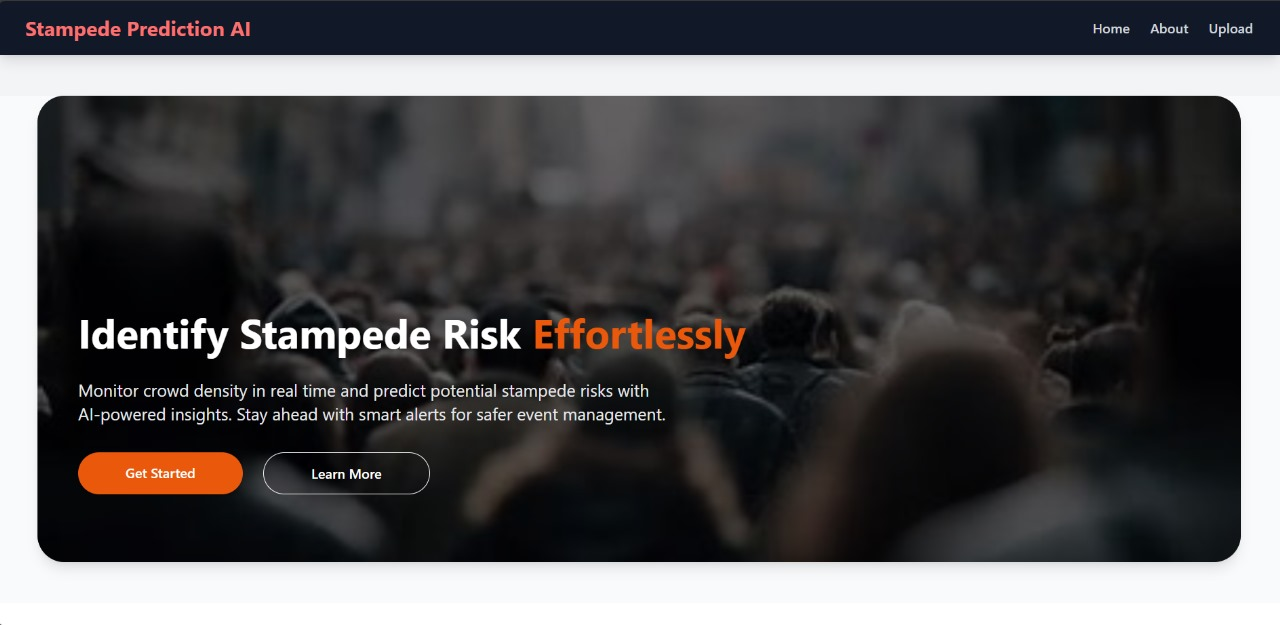
\includegraphics[width=5.8in]{landing.jpg}
      \caption{Landing Page}
    \end{figure} 
    
    \item \textbf{About Page}
        \begin{figure}[H]
          \centering
          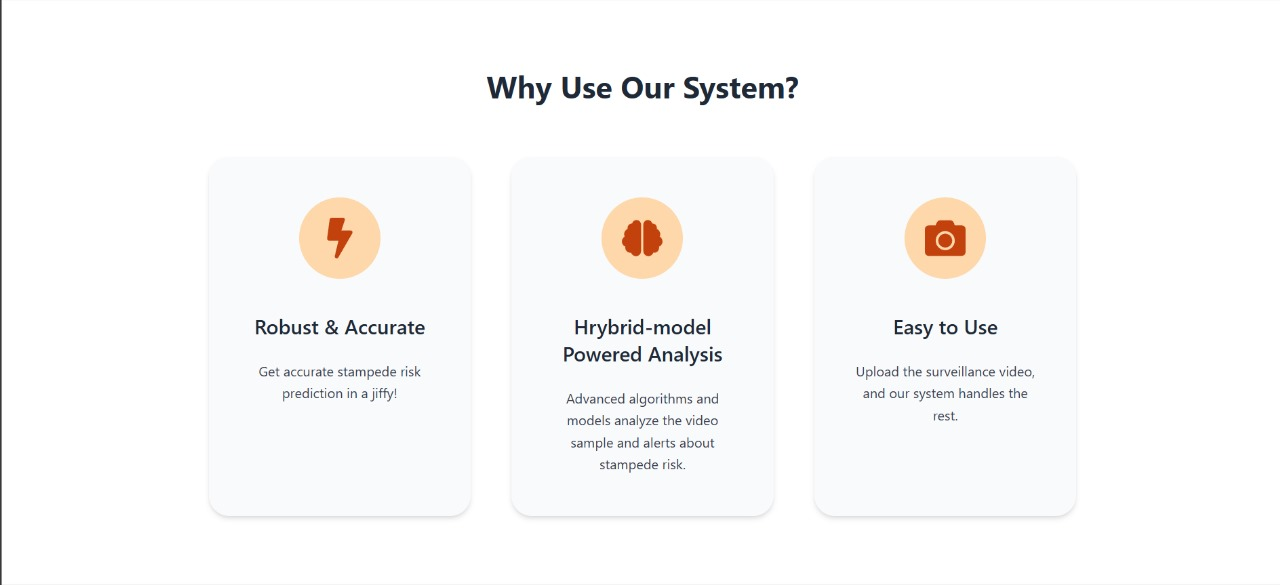
\includegraphics[width=5.8in]{frontend/about1.jpg}
          \caption{About Page}
        \end{figure} 

        \begin{figure}[H]
          \centering
          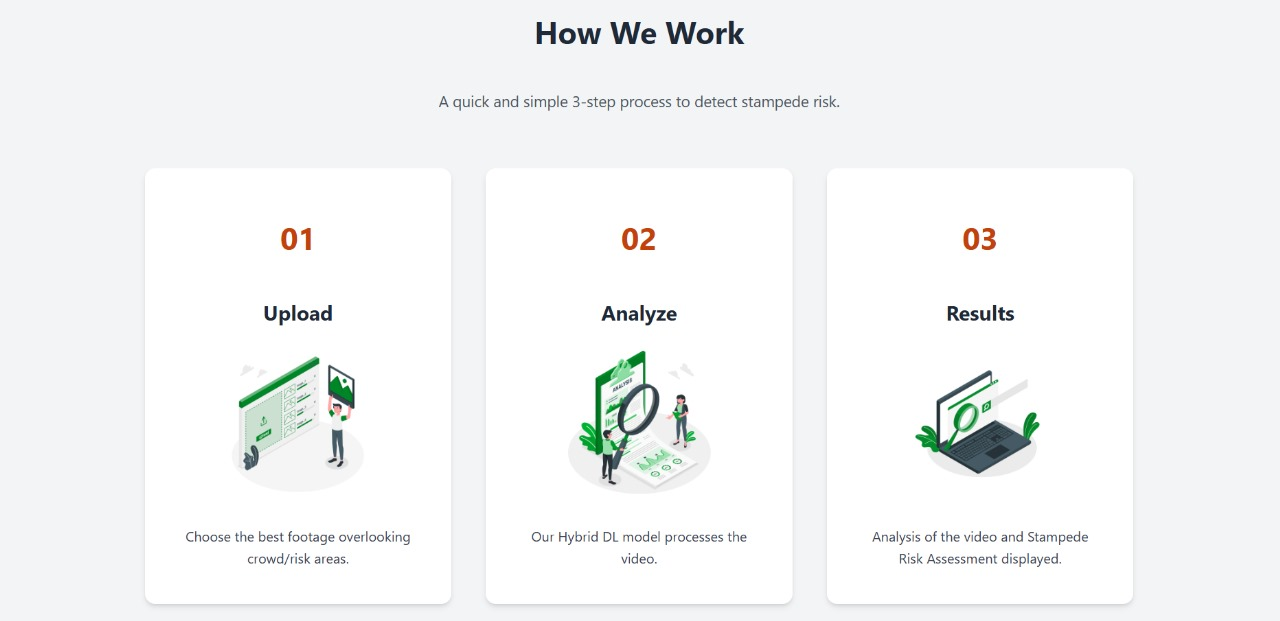
\includegraphics[width=5.8in]{frontend/about2.jpg}
          \caption{About Page}
        \end{figure} 

        \begin{figure}[H]
          \centering
          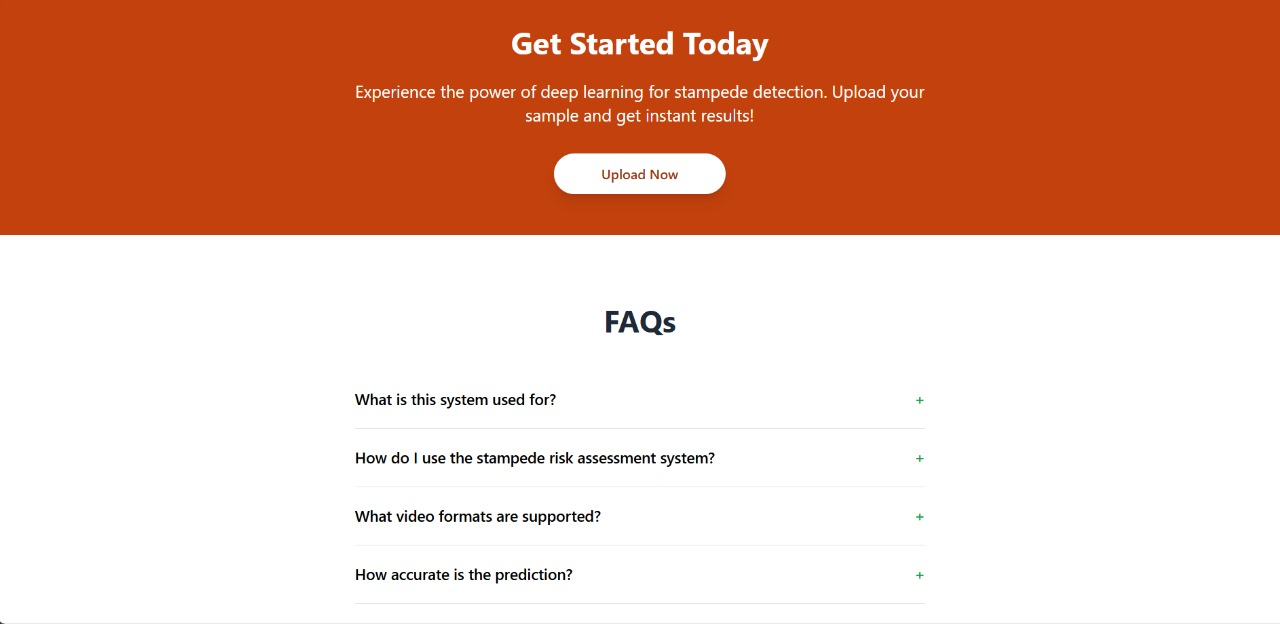
\includegraphics[width=5.8in]{frontend/aboutfaq.jpg}
          \caption{About Page}
        \end{figure} 

    \item \textbf{Upload Page}
        \begin{figure}[H]
          \centering
          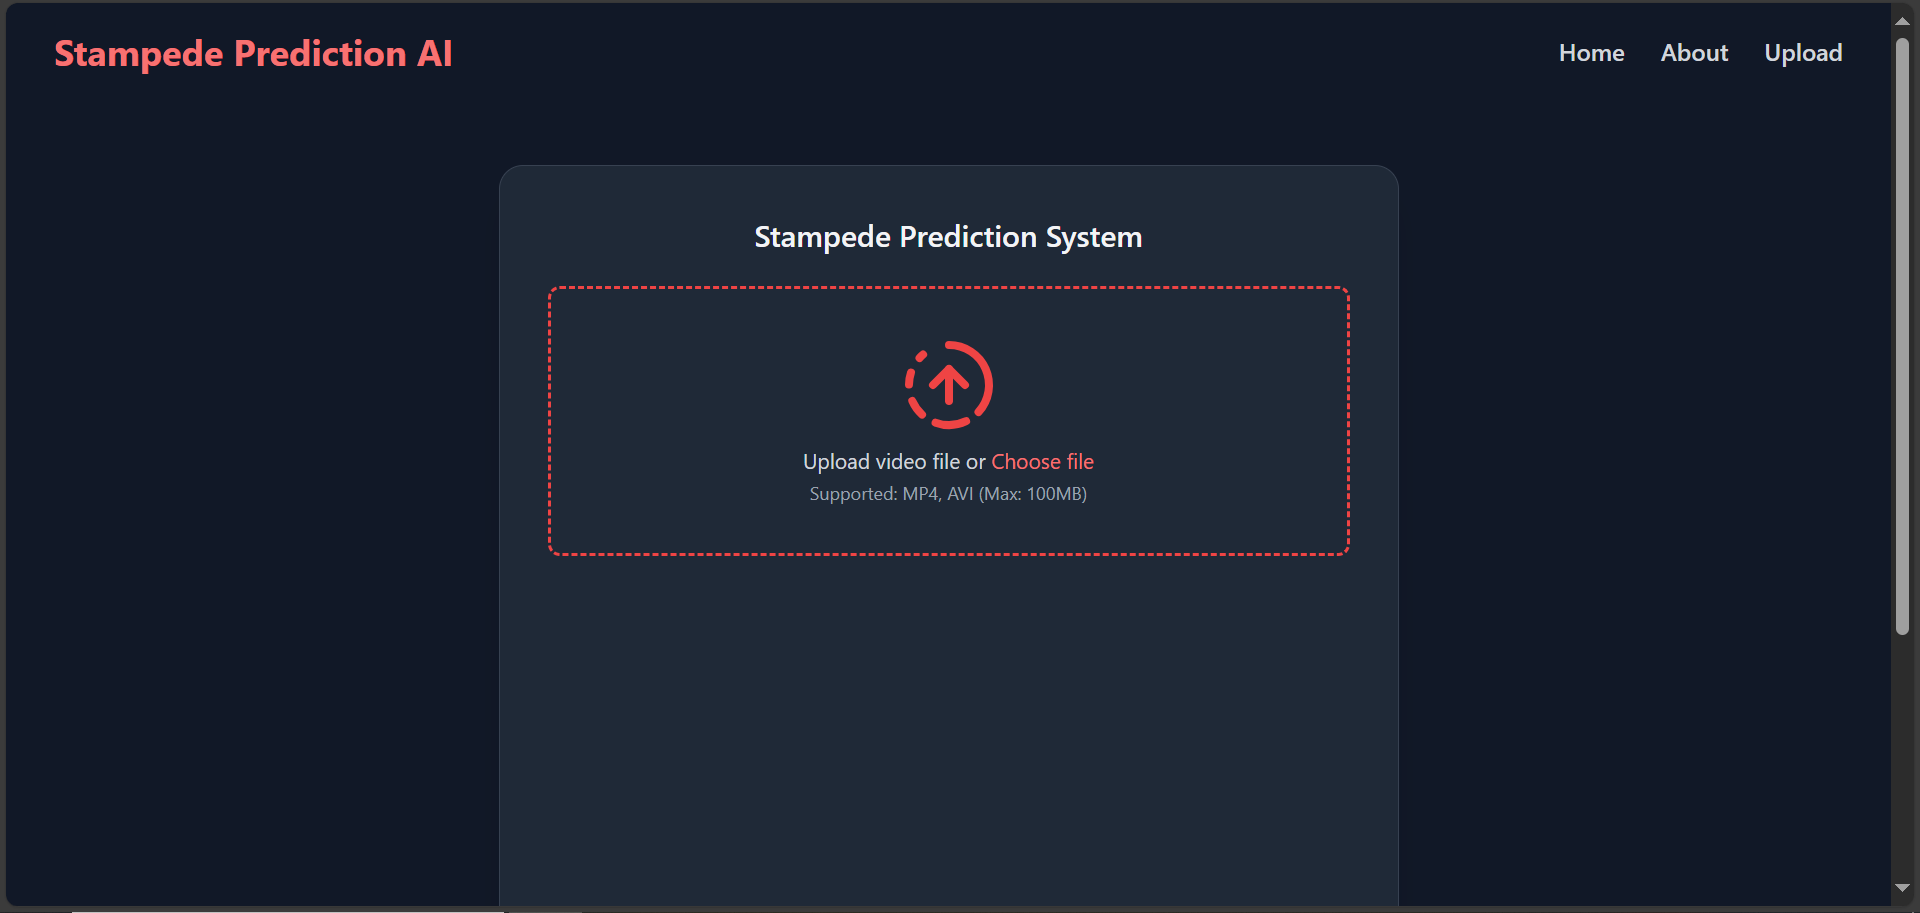
\includegraphics[width=5.8in]{frontend/uploadscreen.png}
          \caption{Upload Page}
        \end{figure} 
        \begin{figure}[H]
          \centering
          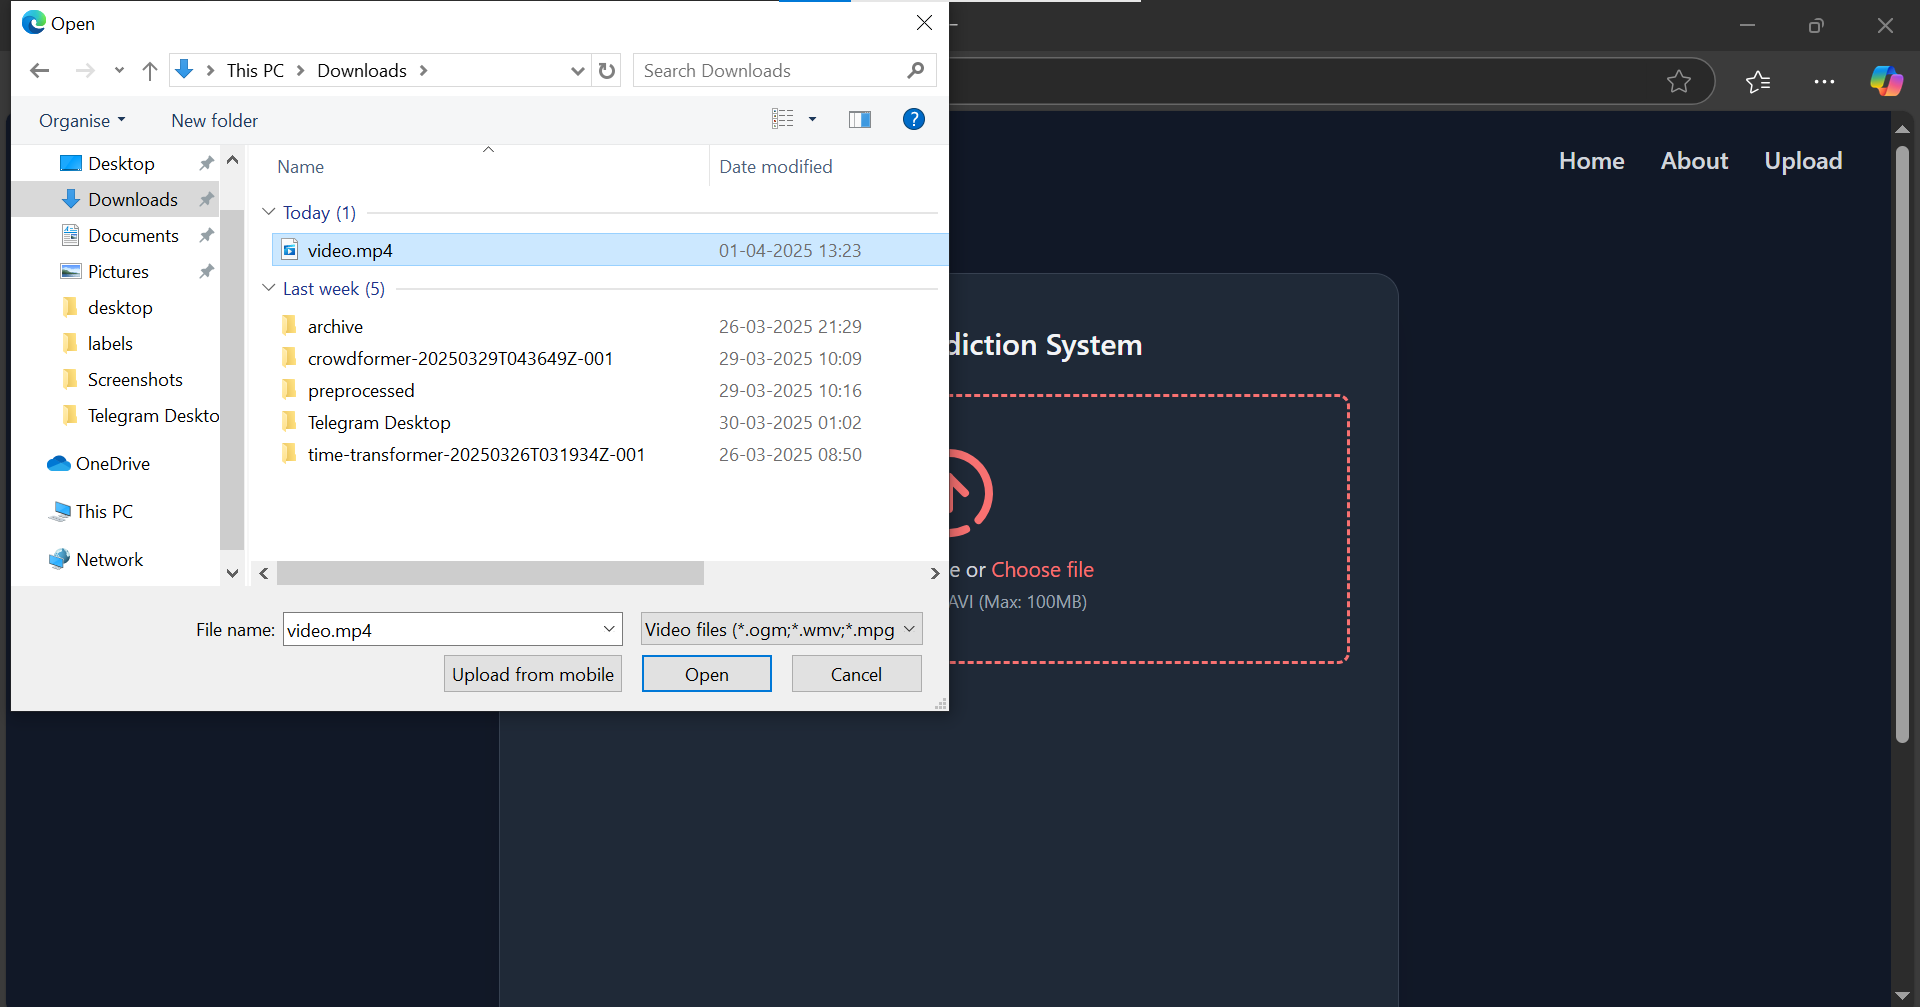
\includegraphics[width=5.8in]{frontend/uploadfileprompt.png}
          \caption{Upload File Prompt}
        \end{figure} 
\end{itemize}

\begin{figure}[H]
          \centering
          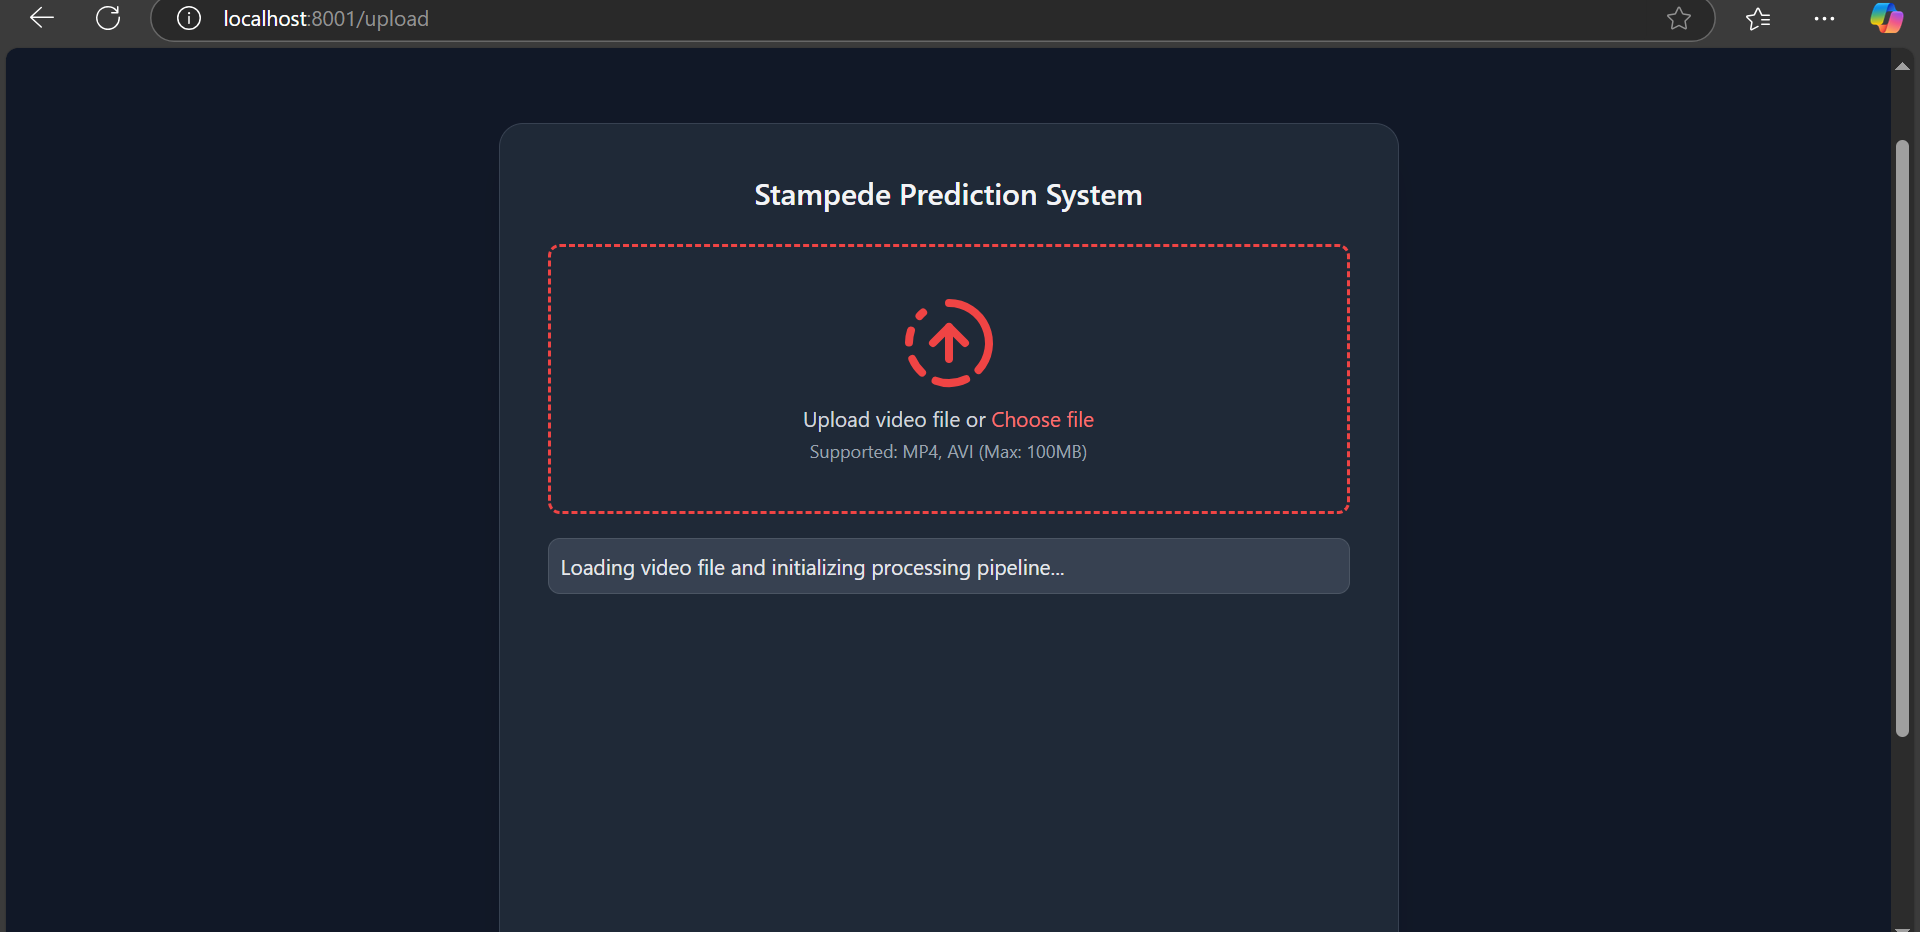
\includegraphics[width=6in]{frontend/loadingmessage.png}
          \caption{Loading Video File in model}
        \end{figure} 

        \begin{figure}[H]
          \centering
          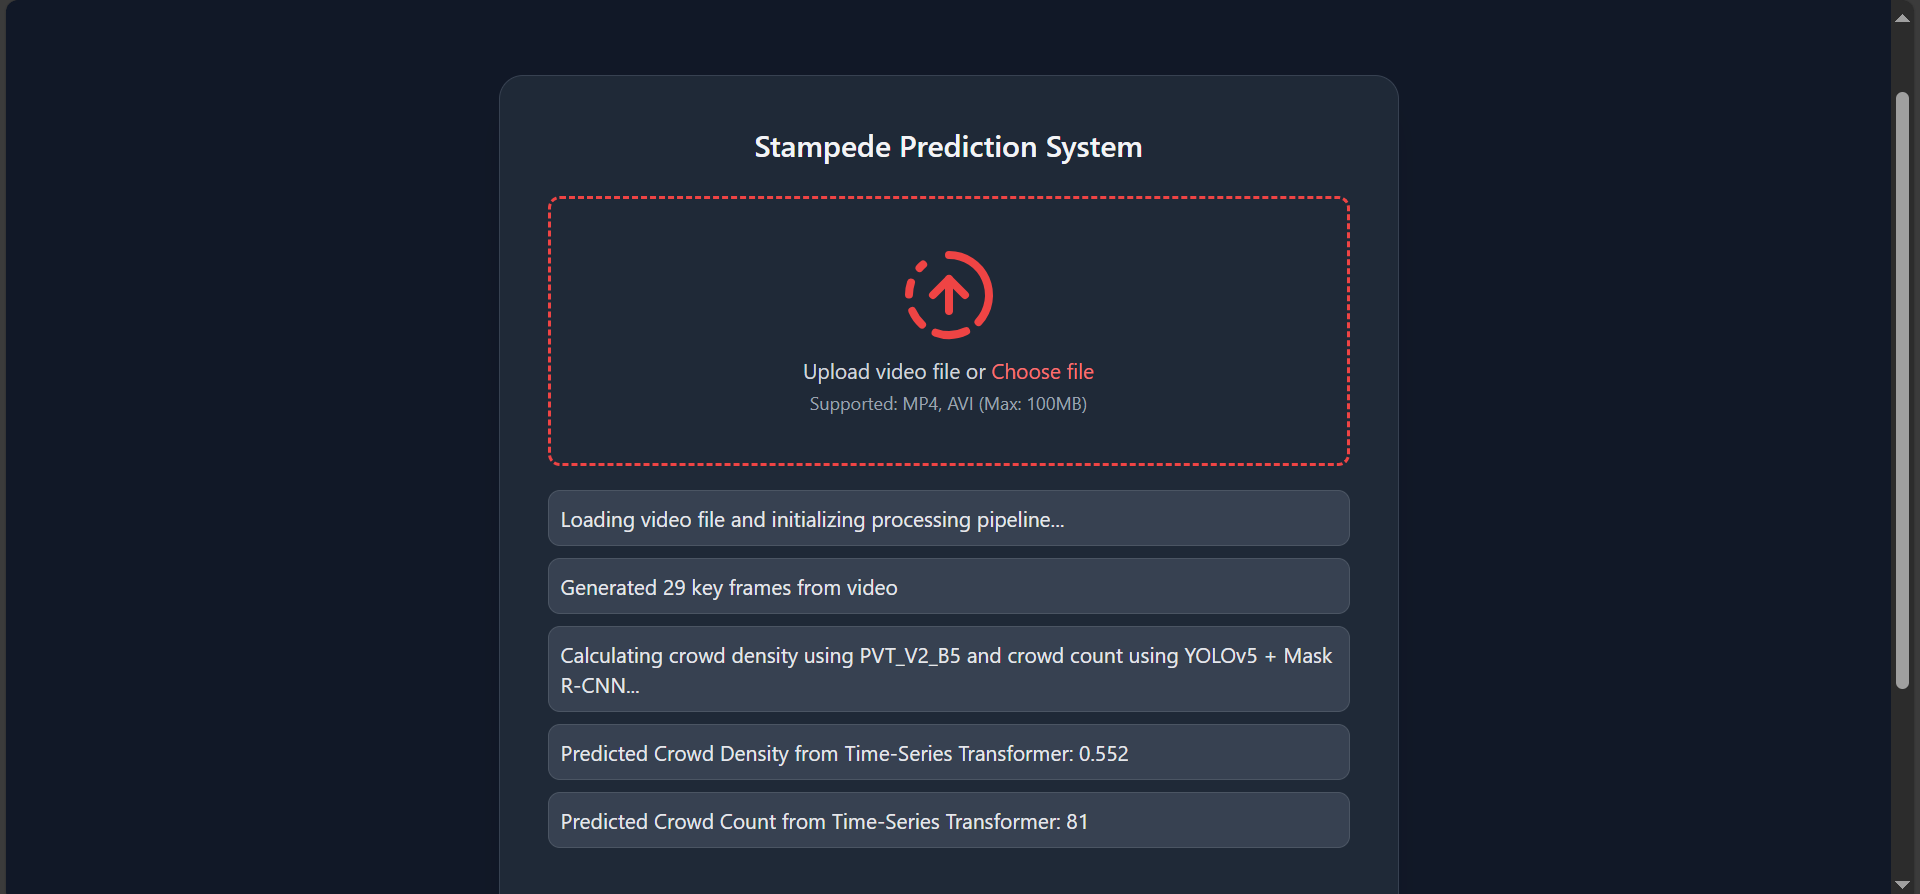
\includegraphics[width=6in]{frontend/step5.png}
          \caption{Crowd Density \&Time-Series Transformer Output Displayed}
        \end{figure} 

        \begin{figure}[H]
          \centering
          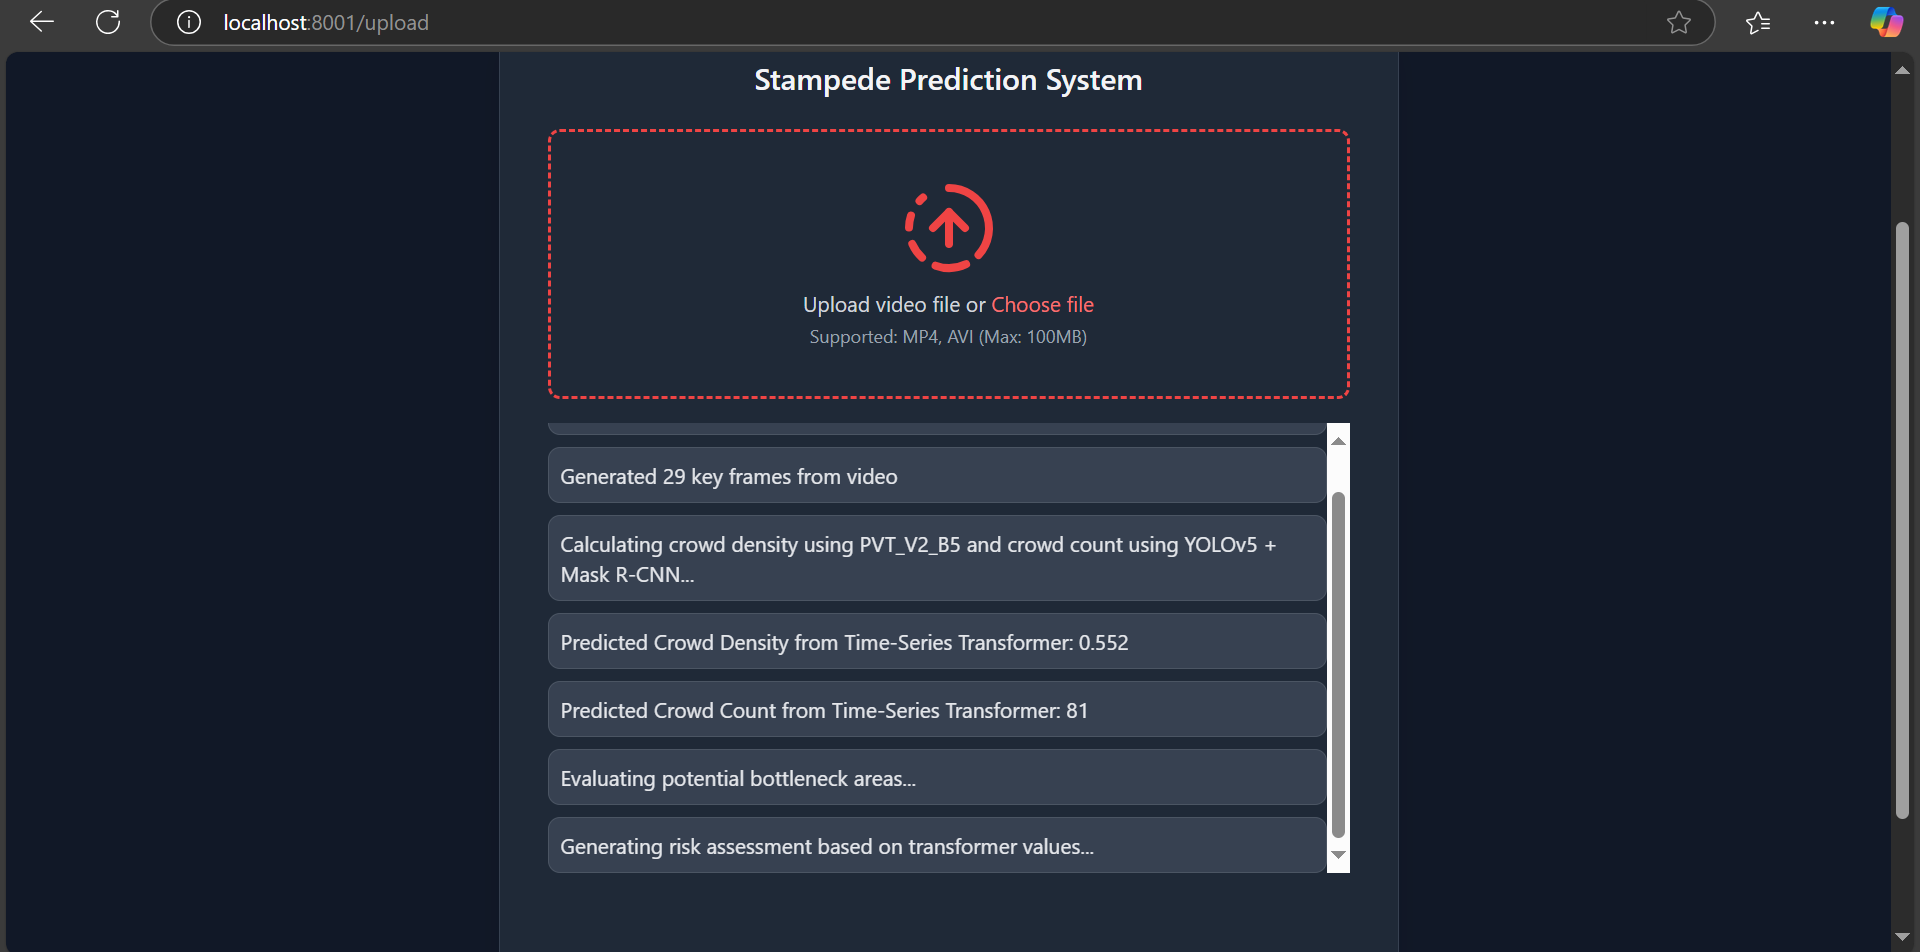
\includegraphics[width=6in]{frontend/Screenshot_2025-04-01_151252.png}
          \caption{UI : Generating Output Loading Message}
        \end{figure} 

        \begin{figure}[H]
          \centering
          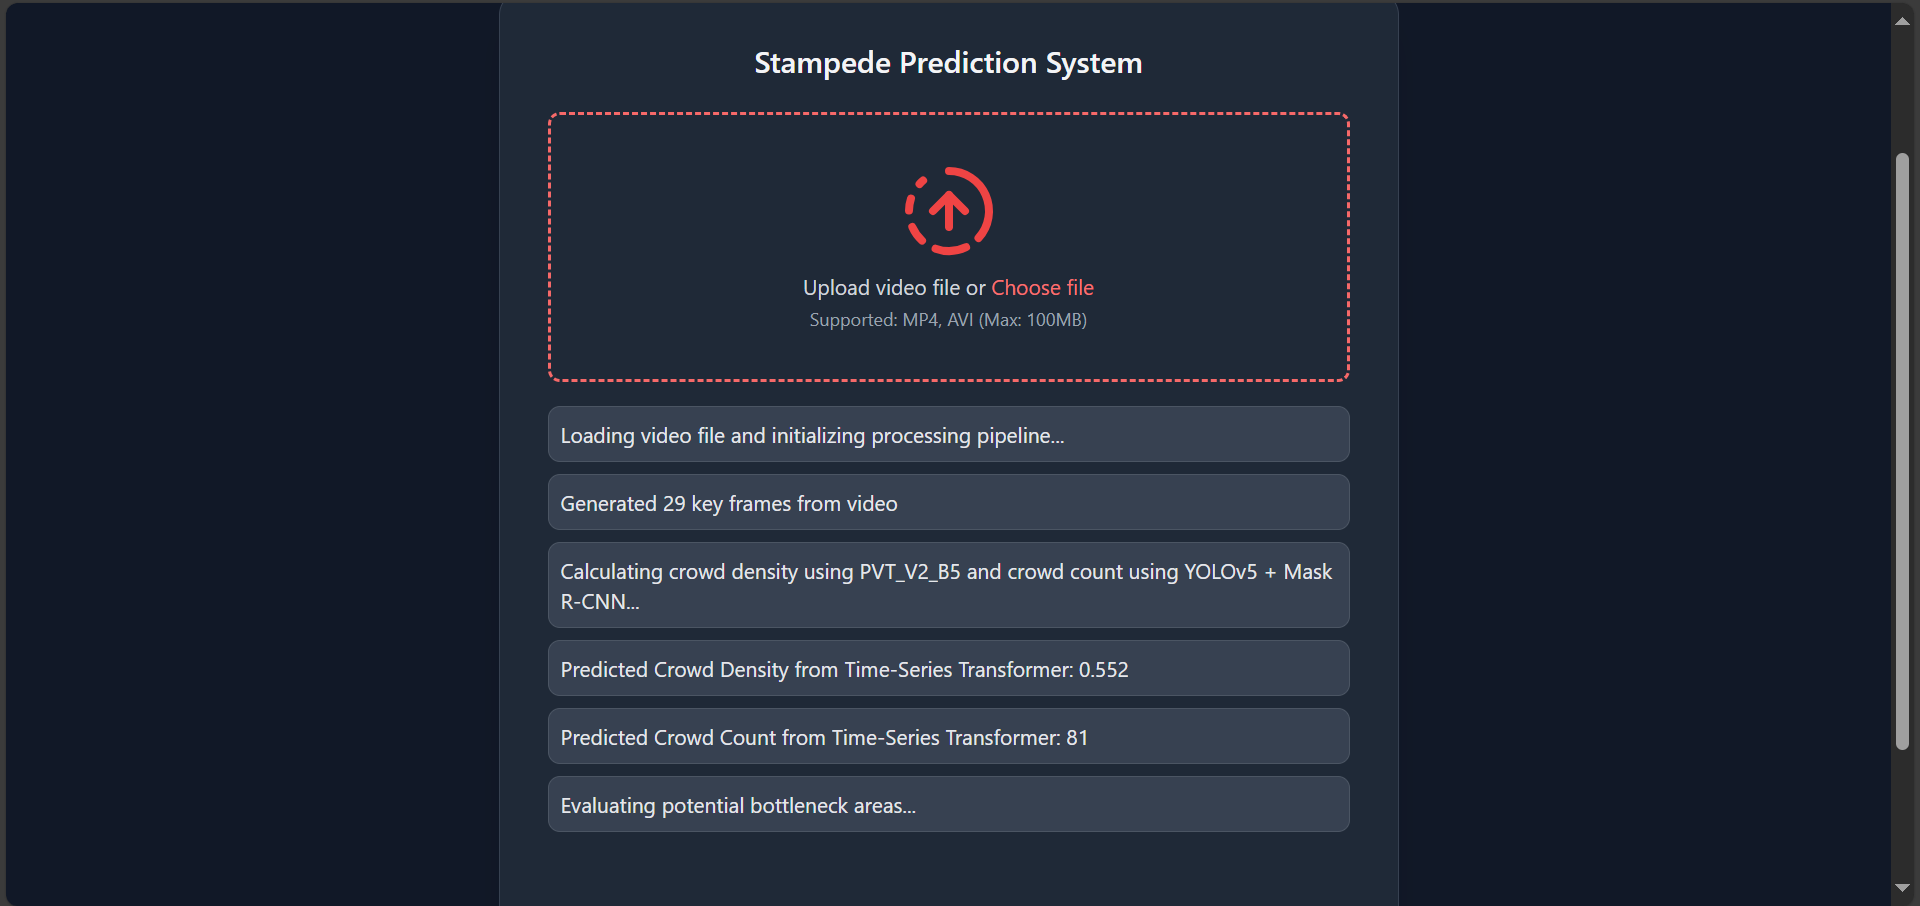
\includegraphics[width=6in]{frontend/6thstep.png}
          \caption{Checking for bottlenecks}
        \end{figure} 

        \begin{figure}[H]
          \centering
          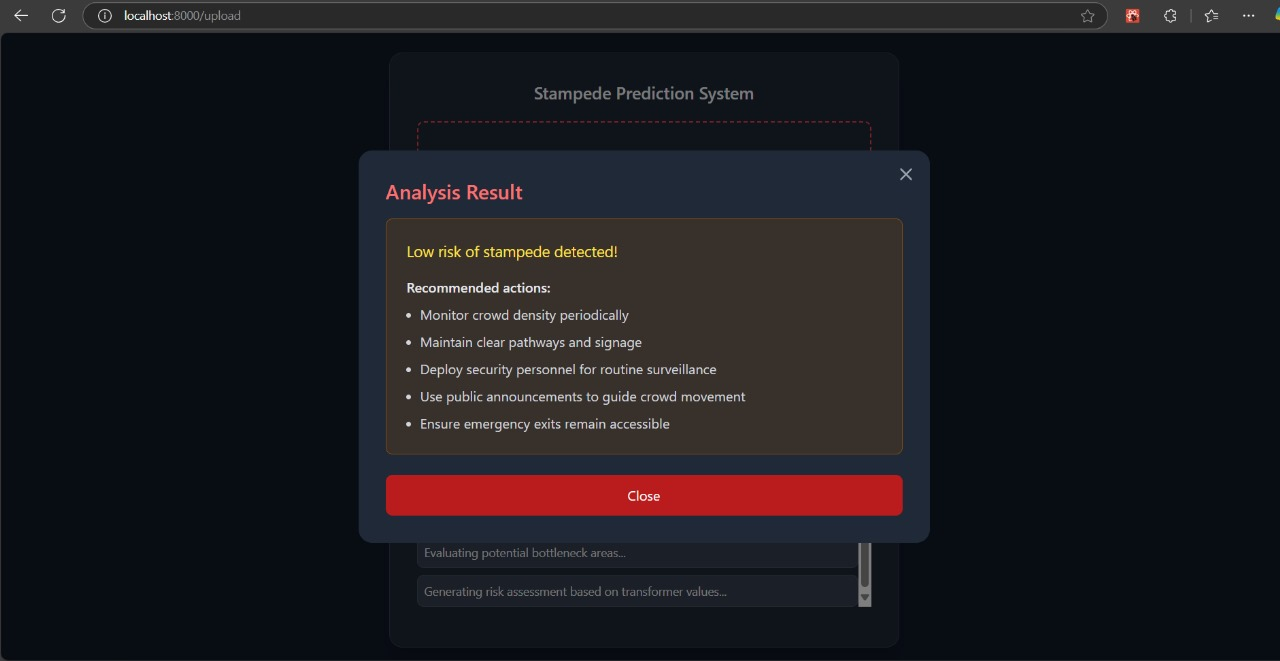
\includegraphics[width=6in]{frontend/lowrisk.jpg}
          \caption{ UI Output : Low Risk of Stampede}
        \end{figure} 
        \begin{figure}[H]
          \centering
          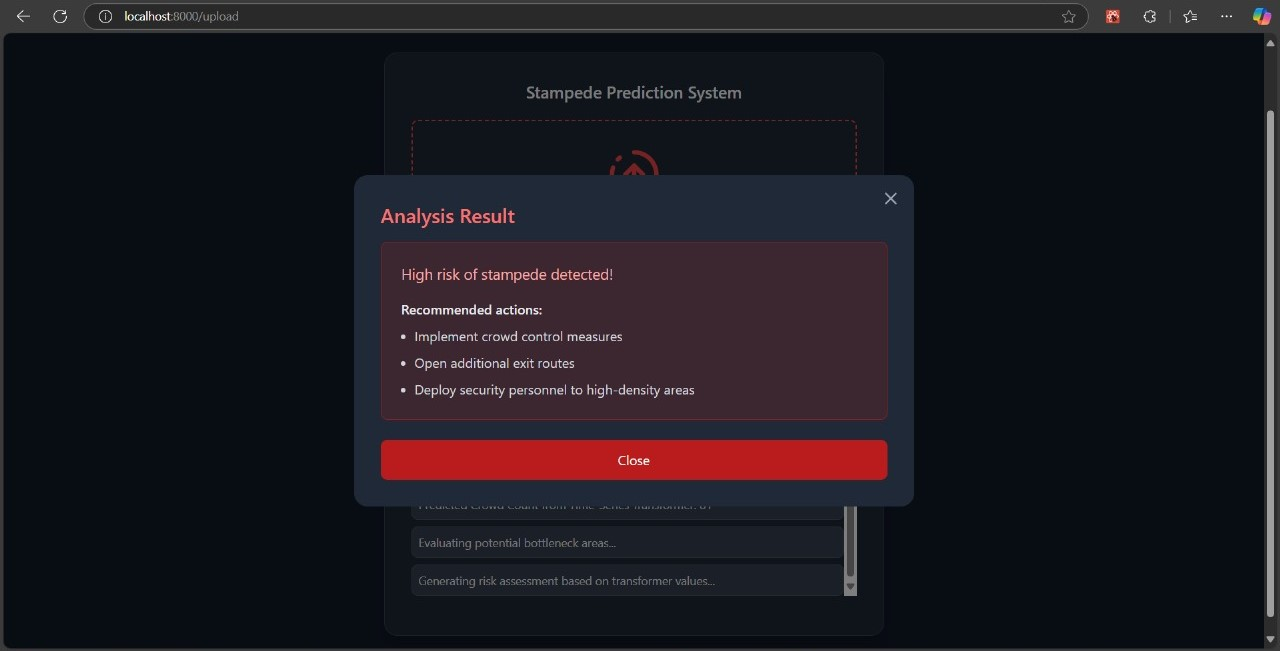
\includegraphics[width=6in]{frontend/highrisk.jpg}
          \caption{ UI Output : High Risk of Stampede}
        \end{figure} 

\chapter{Results \& Analysis}

For our A Hybrid Model for Stampede Detection and Analysis Using YOLOv5, Mask R-CNN, and Time-Series Transformer, which utilizes computing vision, object detection and transformers techniques, extensive testing was conducted to evaluate its effectiveness and usability. The following results were obtained:

\section{System Pipeline}
\subsection{Video processing module results}
\subsubsection{Raw Image Frame}
\begin{figure}[H]
  \centering
  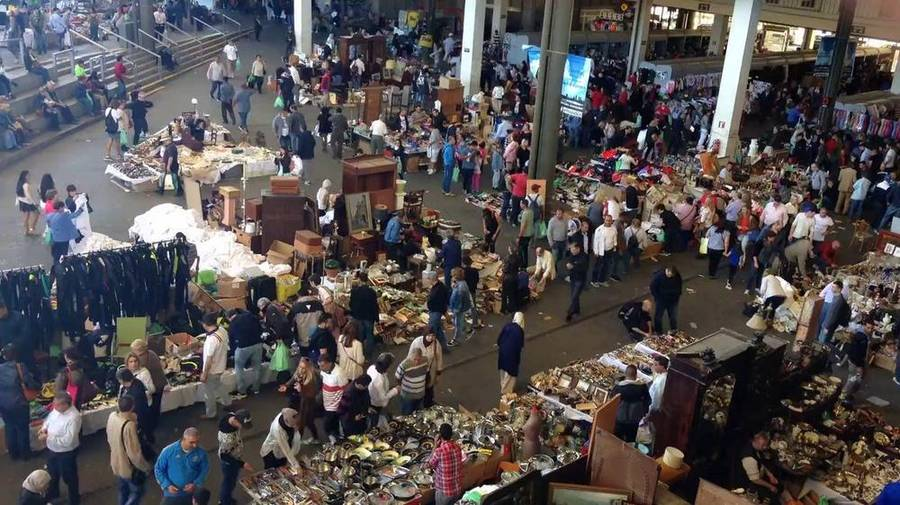
\includegraphics[width=5.5in]{key_frame_0000.jpg}
  \caption{Raw Image Frame}
\end{figure}

% \subsection{Sampled Image Frame}
% \begin{figure}[H]
%   \centering
%   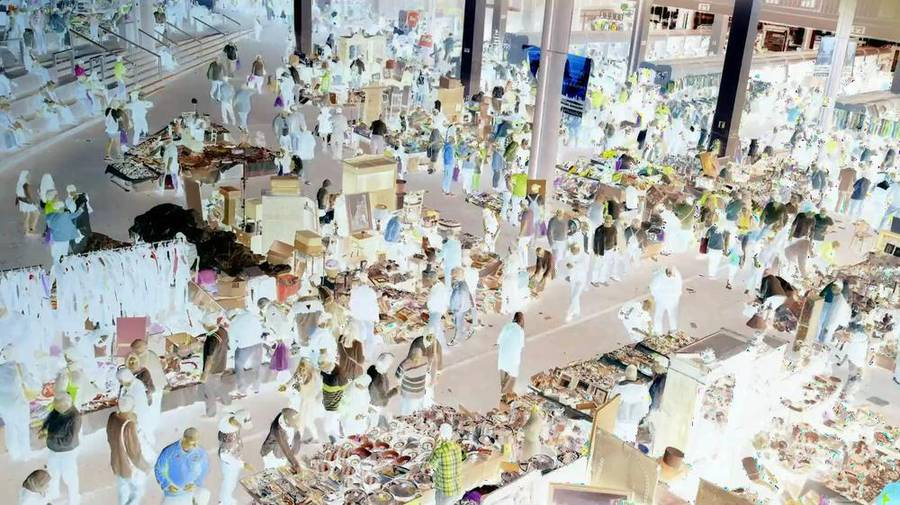
\includegraphics[width=5.5in]{sampled_frame_0000.jpg}
%   \caption{Sampled Image Frame}
% \end{figure}

\begin{comment}
\begin{figure}[H]
  \centering
  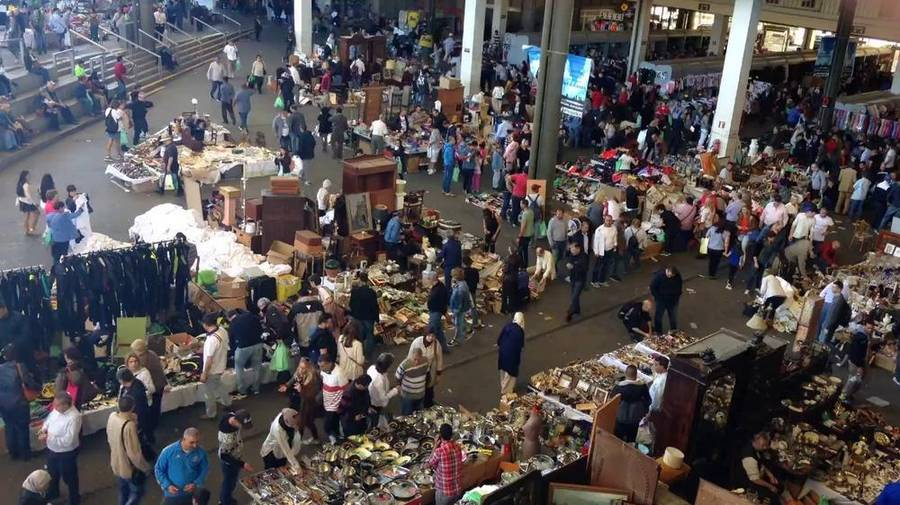
\includegraphics[width=6in]{key-farme.jpg}
  \caption{Key}
\end{figure}
\end{comment}

\subsubsection{Extracted Key Image Frame}
\begin{figure}[H]
  \centering
  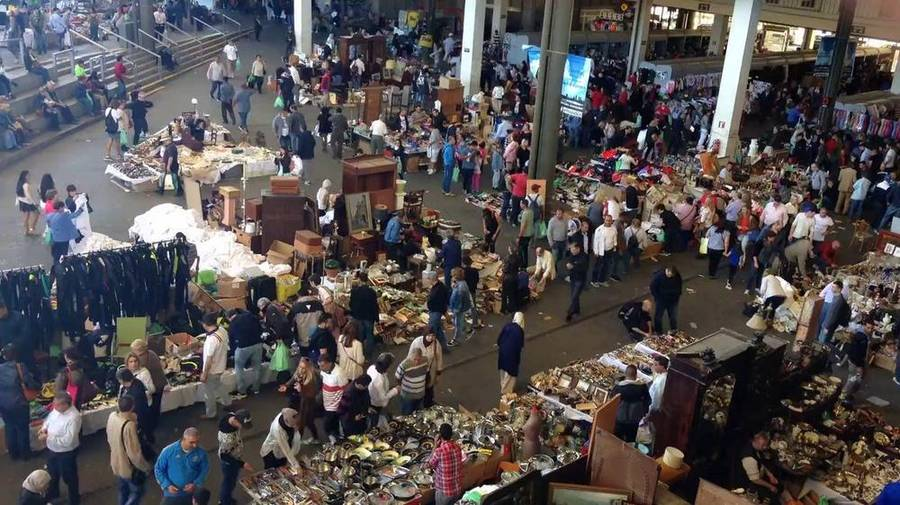
\includegraphics[width=5.5in]{key_frame_0000.jpg}
  \caption{Key Image Frame}
\end{figure}

\subsubsection{Denoised Image Frame}
\begin{figure}[H]
  \centering
  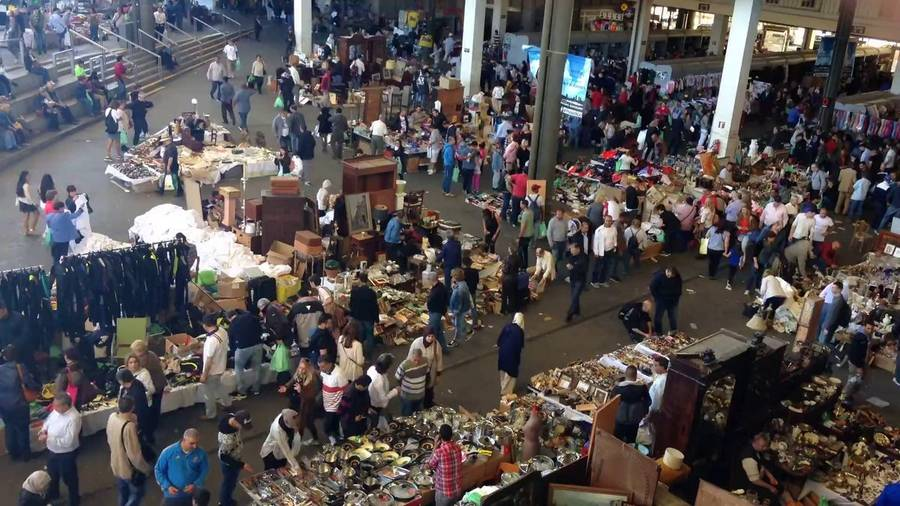
\includegraphics[width=5.5in]{denoised_frame_0000.jpg}
  \caption{Denoised Image Frame}
\end{figure}

% \begin{figure}[H]
%   \centering
%   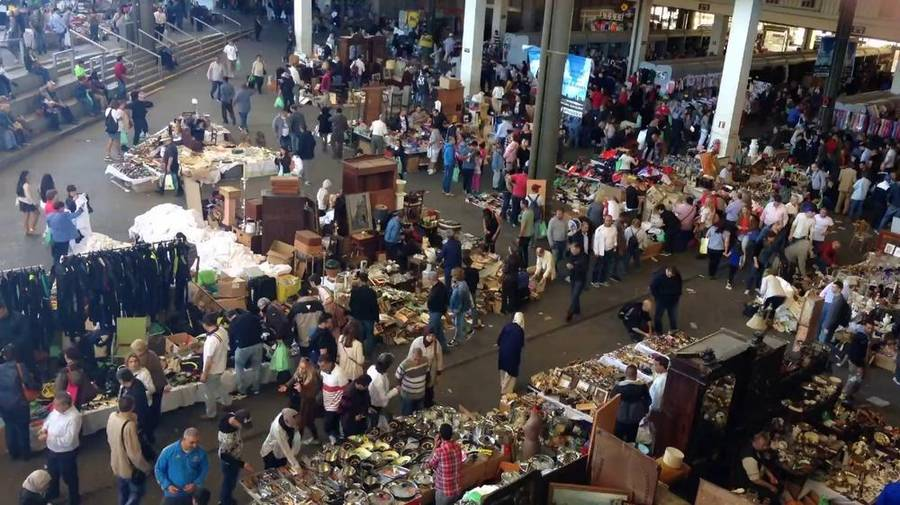
\includegraphics[width=5.5in]{denoised.jpg}
%   \caption{Denoise}
% \end{figure}

\begin{comment}
\begin{figure}[H]
  \centering
  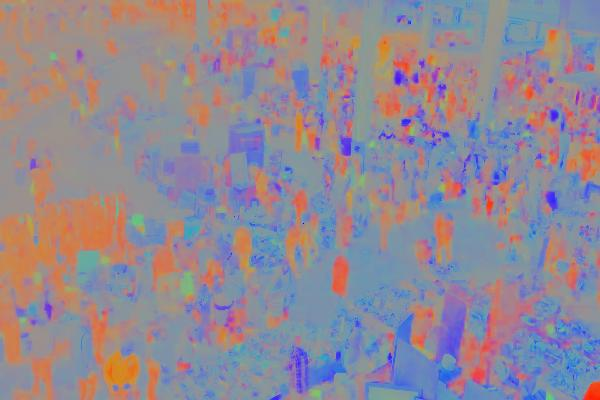
\includegraphics[width=6in]{normalized_frame_0000.jpg}
  \caption{nromalised}
\end{figure}
\end{comment}

\subsubsection{Preprocessed Image Frame}
% \begin{figure}[H]
%   \centering
%   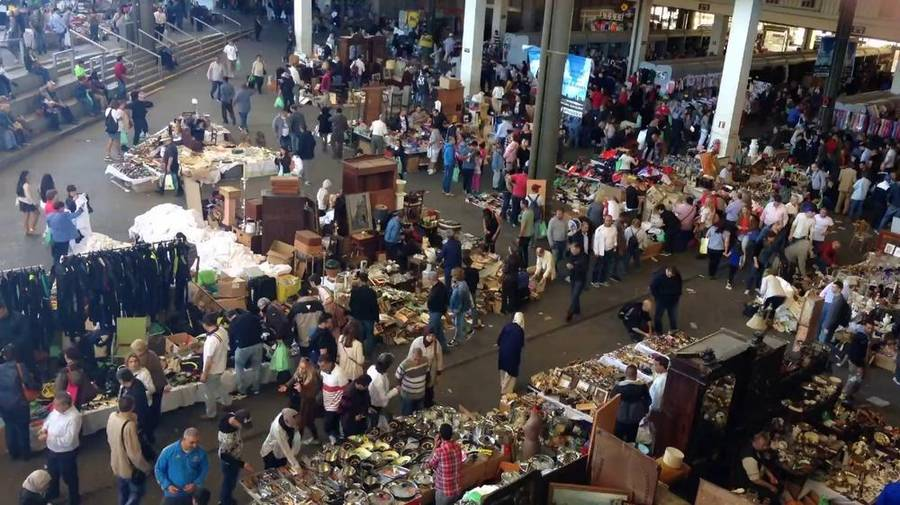
\includegraphics[width=5.5in]{preprocessed.jpg}
%   \caption{Preprocessed Image Frame}
% \end{figure}


\begin{figure}[H]
  \centering
  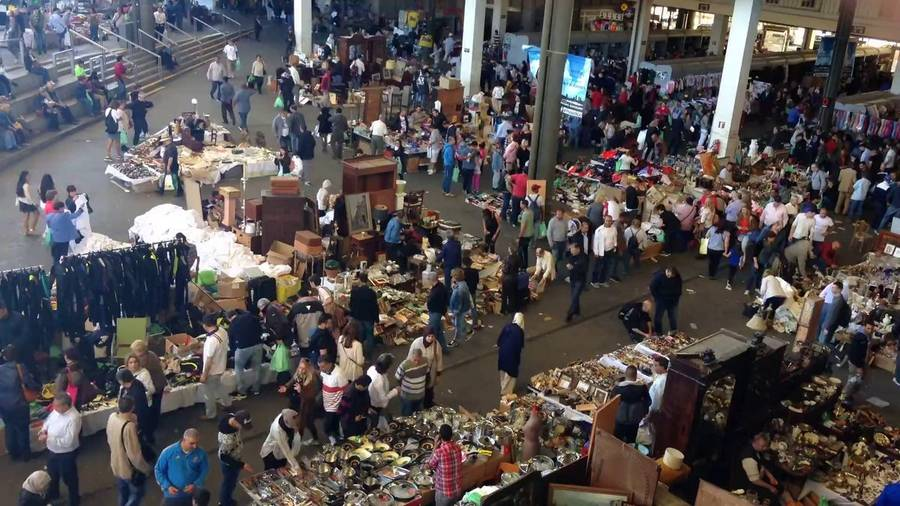
\includegraphics[width=5.5in]{preprocessed_frame_0000.jpg}
  \caption{Preprocessed Image Frame}
\end{figure}



\begin{comment}
\begin{figure}[H]
  \centering
  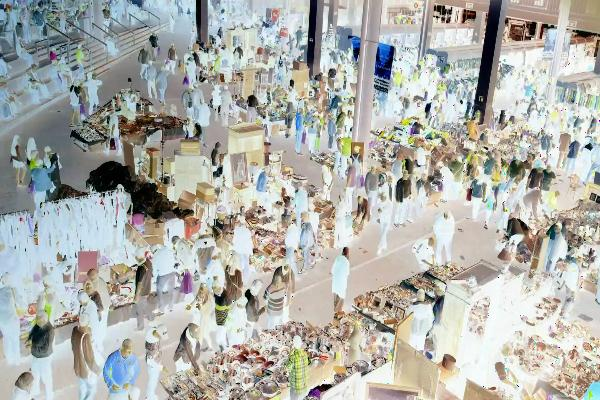
\includegraphics[width=6in]{resized_frame_0000.jpg}
  \caption{resized frame}
\end{figure}
\end{comment}

\begin{comment}
\begin{figure}[H]
  \centering
  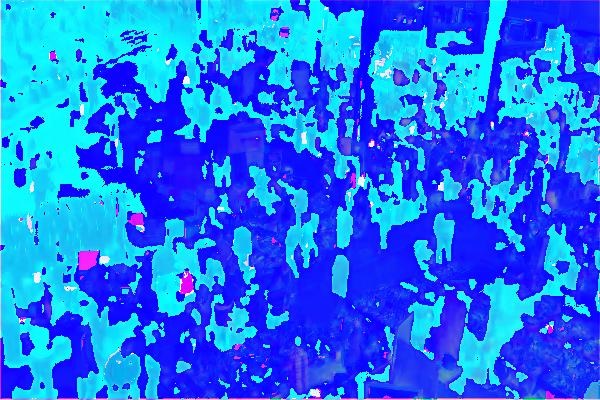
\includegraphics[width=6in]{skip_frame_0000.jpg}
  \caption{Skip Frame}
\end{figure}
\end{comment}

\section{Crowd Monitoring Results}
\begin{figure}[H]
  \centering
  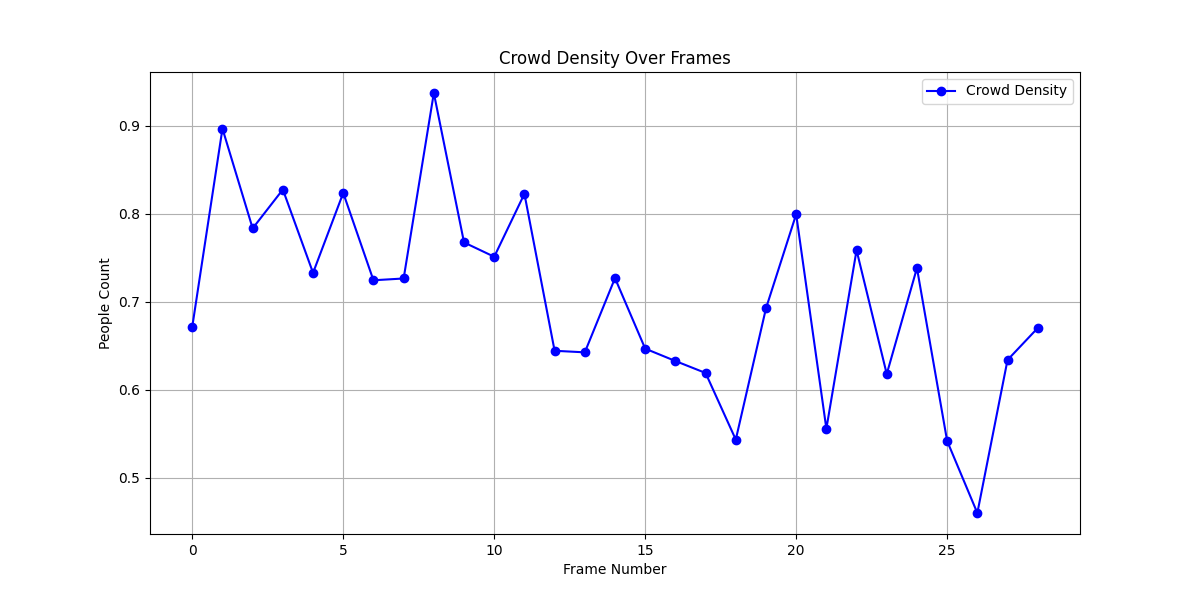
\includegraphics[width=6in]{crowd_density_trend.png}
  \caption{Graph of Crowd Density Trend}
\end{figure}

\section{Crowd Counting}
\subsection{Mask R-CNN}
\begin{figure}[H]
  \centering
  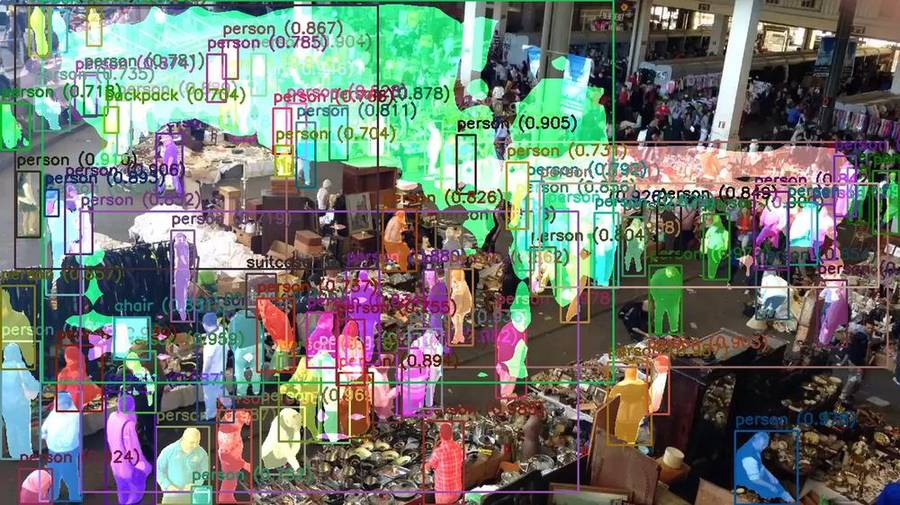
\includegraphics[width=6in]{maskrcnn.jpg}
  \caption{People detected by Mask R-CNN}
\end{figure}


\begin{figure}[H]
  \centering
  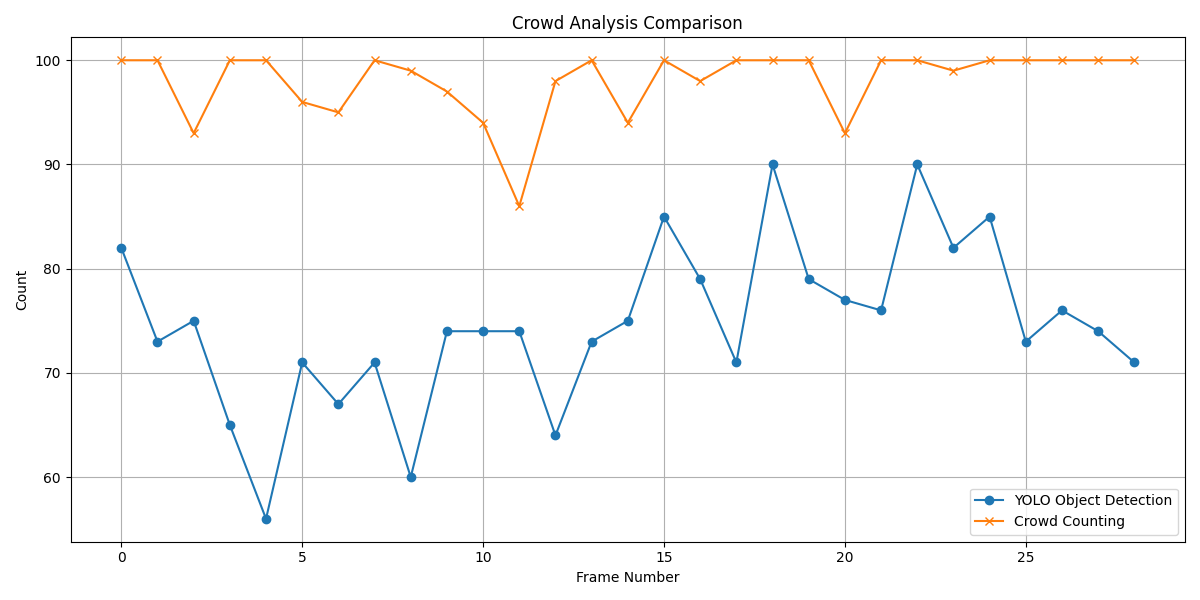
\includegraphics[width=6in]{crowd_analysis_comparison.png}
  \caption{Graph of Crowd Analysis : Transformer vs YOLOv5}
\end{figure}

\begin{figure}[H]
  \centering
  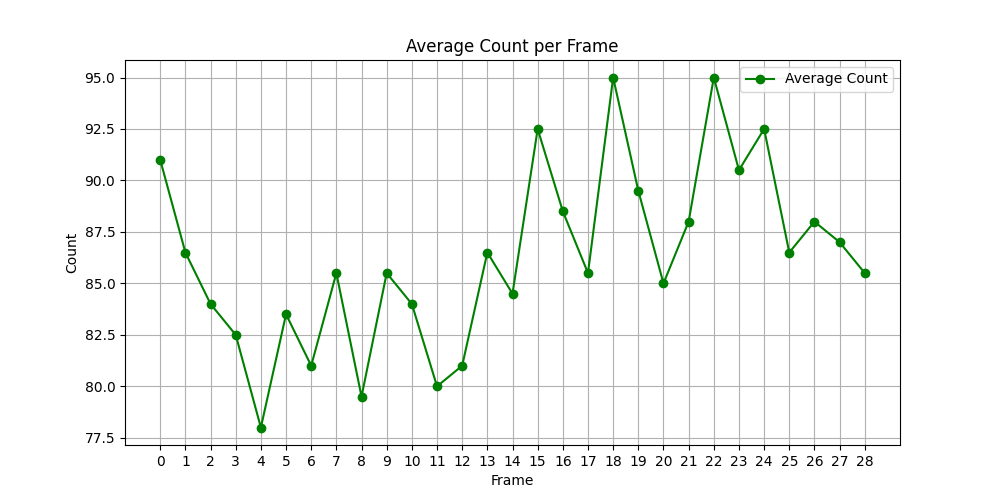
\includegraphics[width=6in]{avg_count.png}
  \caption{Graph : Average Count per Frame}
\end{figure}

\section{Stampede Detection Module}

\begin{figure}[H]
    \centering
    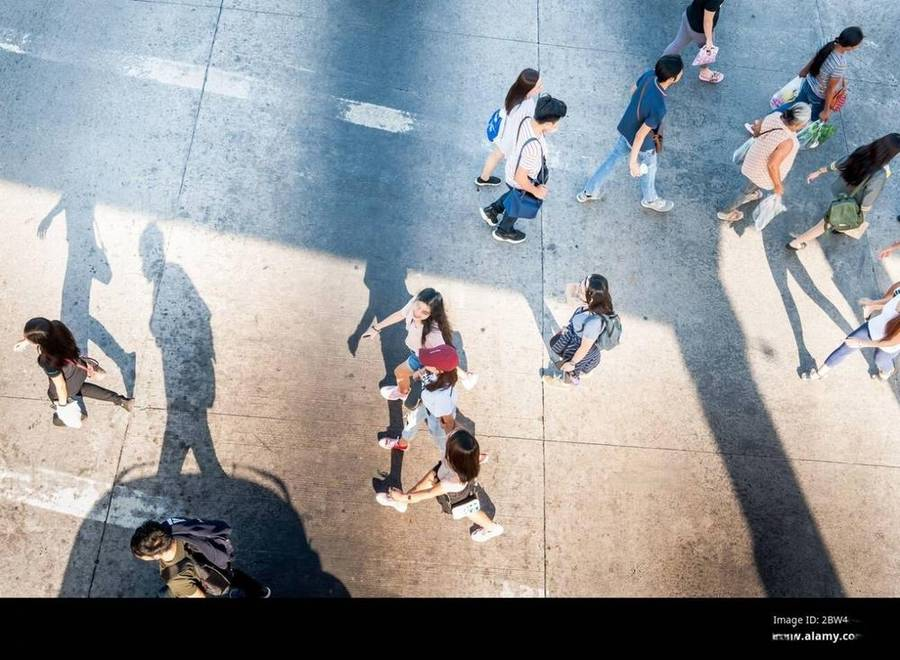
\includegraphics[width=0.75\linewidth]{verylowrisk.jpg}
    \caption{Image of Low Risk Stampede}
\end{figure}
\begin{figure}[H]
    \centering
    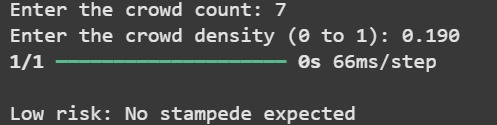
\includegraphics[width=0.75\linewidth]{stampedelowrisk.jpg}
    \caption{Output : Low Risk, No Stampede}
\end{figure}

\begin{comment}
\begin{figure}[H]
    \centering
    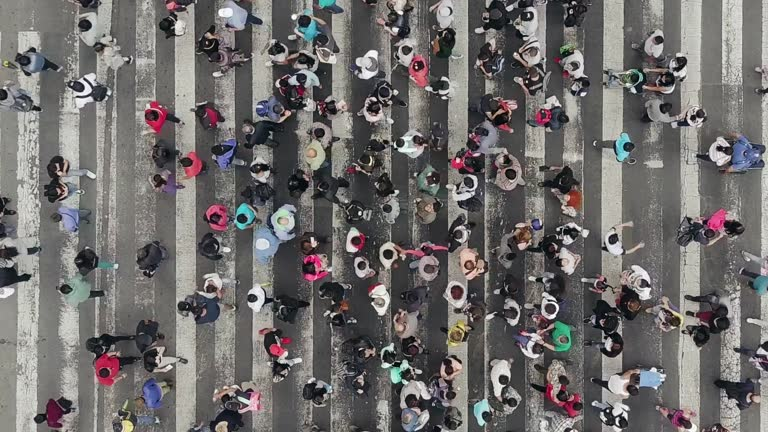
\includegraphics[width=0.85\linewidth]{lowriskstampedeimg.jpg}
    \caption{Image of Low Risk Stampede}
\end{figure}
\end{comment}
\begin{figure}[H]
    \centering
    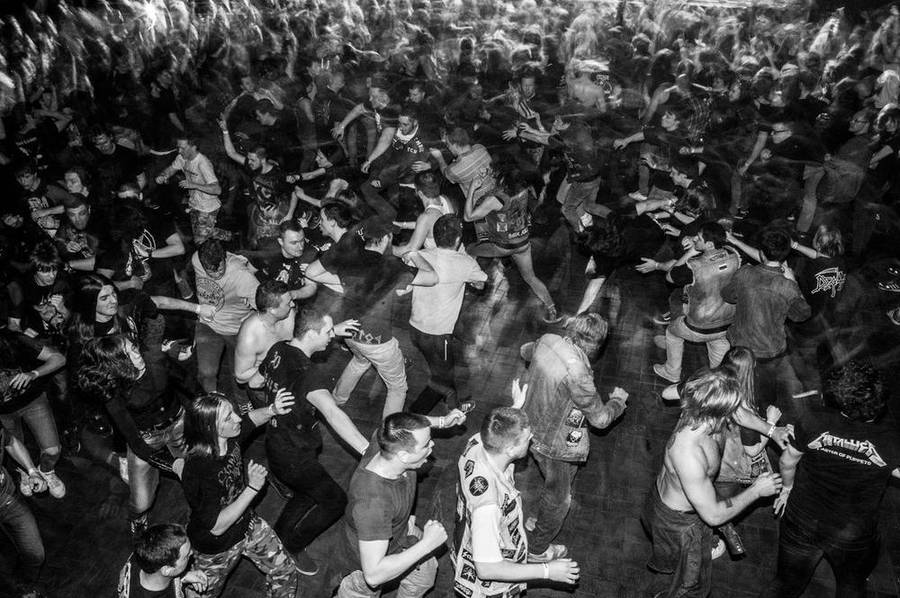
\includegraphics[width=0.75\linewidth]{stampedelowlight.jpg}
    \caption{Input : Image of Stampede, in Low Light Conditions}
\end{figure}

\begin{figure}[H]
    \centering
    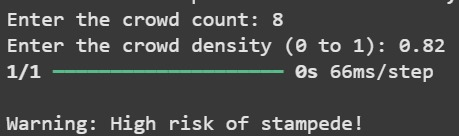
\includegraphics[width=0.75\linewidth]{highriskstampede.jpg}
    \caption{Output : High Risk of Stampede}
\end{figure}

\begin{comment}
    

\begin{figure}[H]
    \centering
    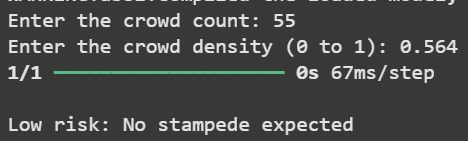
\includegraphics[width=0.75\linewidth]{lowriskstampede.jpg}
    \caption{Enter Caption}
\end{figure}

\begin{figure}[H]
    \centering
    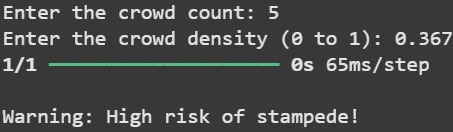
\includegraphics[width=0.75\linewidth]{stampedehighrisk.jpg}
    \caption{Enter Caption}
\end{figure}
\end{comment}

\begin{figure}[H]
  \centering
  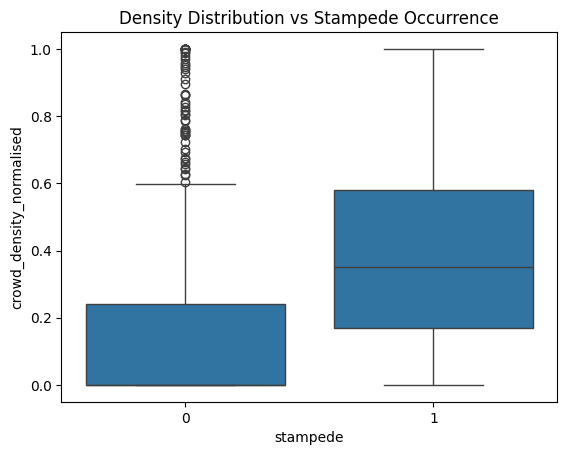
\includegraphics[width=5in]{density_distribution_vs_stampede_occurance.png}
  \caption{Graph : Density vs Stampede Occurance}
\end{figure}

\section{Evaluation Metrics}
To assess the performance and reliability of the stampede detection system, the following evaluation metrics are used for assessing logistics regression model and other models used:

\begin{itemize}
     \item \textbf{Accuracy}: Measures the overall correctness of the model by evaluating the proportion of correctly classified instances among all instances. It is defined as:
    \begin{equation}
        \text{Accuracy} = \frac{TP + TN}{TP + TN + FP + FN}
    \end{equation}
    where $TN$ denotes True Negatives. A higher accuracy value indicates better overall performance in distinguishing between positive and negative cases.
    
\begin{figure}[H]
    \centering
    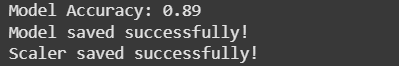
\includegraphics[width=5in]{modelaccuracy.png}
    \caption{Model Accuracy}
\end{figure}
\begin{comment}
    \item \textbf{Intersection over Union (IoU)}: Measures the accuracy of object localization by calculating the overlap between the predicted bounding box and the ground truth bounding box. It is defined as:
    \begin{equation}
        IoU = \frac{\text{Area of Overlap}}{\text{Area of Union}}
    \end{equation}
    A higher IoU value indicates better localization.
\end{comment}
    \item \textbf{Confusion Matrix}: A performance evaluation tool for classification models that summarizes the number of correct and incorrect predictions across different classes. It consists of four key components:  
    \begin{itemize}
        \item \textbf{True Positives (TP)}: Cases where the model correctly predicts the positive class.  
        \item \textbf{True Negatives (TN)}: Cases where the model correctly predicts the negative class.  
        \item \textbf{False Positives (FP)}: Cases where the model incorrectly predicts the positive class (also known as Type I Error).  
        \item \textbf{False Negatives (FN)}: Cases where the model incorrectly predicts the negative class (also known as Type II Error).  
    \end{itemize}
    The confusion matrix provides insights into model accuracy, precision, recall, and overall classification performance.
\begin{figure}[H]
    \centering
    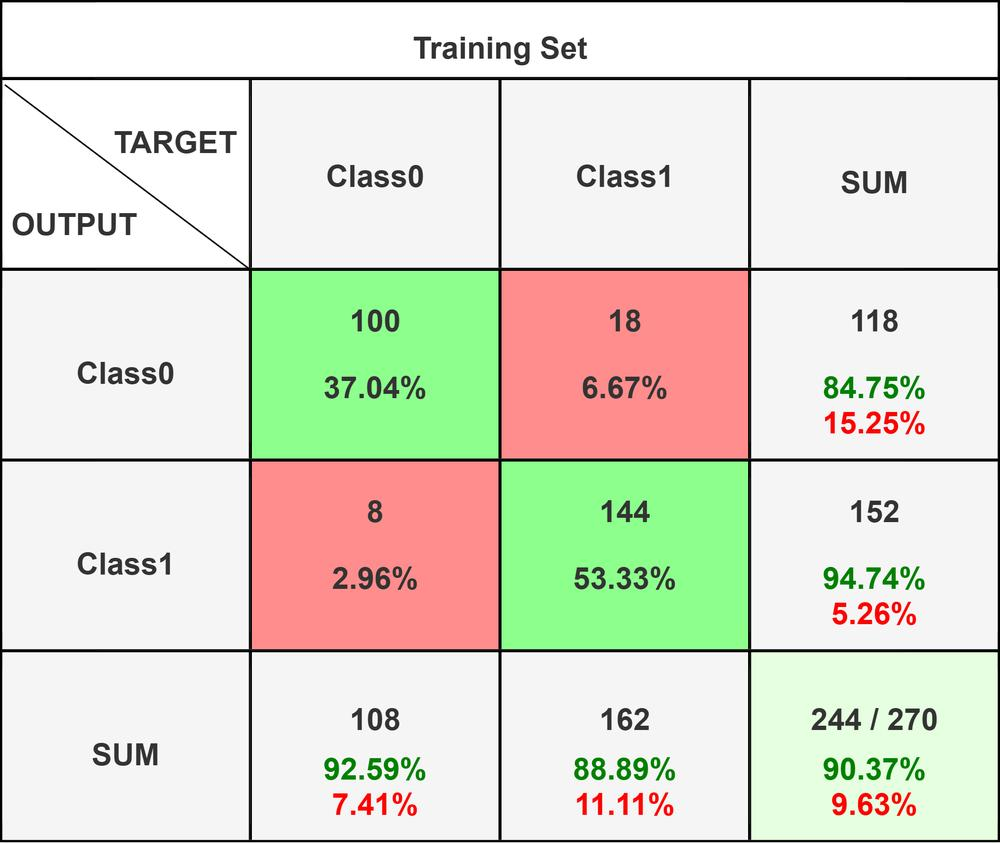
\includegraphics[width=0.75\linewidth]{Confusion_Matrix.jpg}
    \caption{Confusion Matrix}
\end{figure}
    \item \textbf{ROC - AUC}: The Receiver Operating Characteristic (ROC) curve is a graphical representation of a classification model’s performance across different threshold values. It plots the True Positive Rate (TPR) against the False Positive Rate (FPR), showing the trade-off between sensitivity and specificity.  
    \begin{equation}
        \text{TPR} = \frac{\text{TP}}{\text{TP} + \text{FN}}, \quad
        \text{FPR} = \frac{\text{FP}}{\text{FP} + \text{TN}}
    \end{equation}
    The \textbf{Area Under the Curve (AUC)} quantifies the overall performance of the classifier. A higher AUC value (closer to 1) indicates a better-performing model, while an AUC of 0.5 suggests a random classifier.  
   \begin{figure}[H]
        \centering
        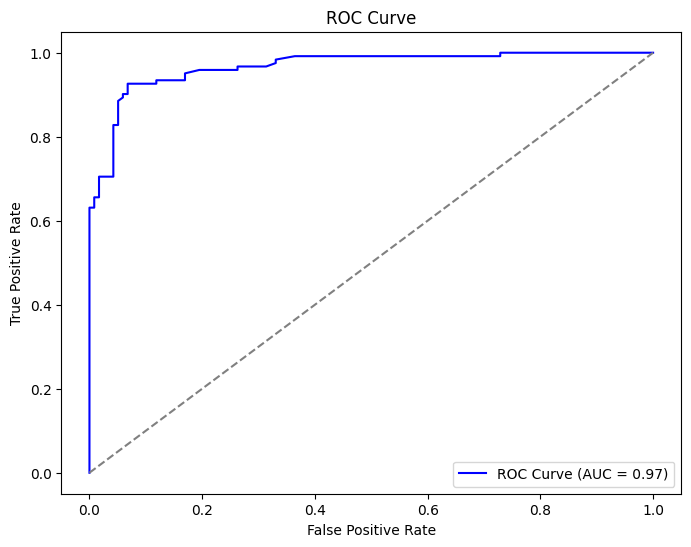
\includegraphics[width=0.75\linewidth]{roc-final.png}
        \caption{ROC-AUC Curve}
    \end{figure}
    \item \textbf{Precision}: Represents the proportion of correctly identified detections among all detections made. It is calculated as:
    \begin{equation}
        \text{Precision} = \frac{TP}{TP + FP}
    \end{equation}
    where $TP$ denotes True Positives and $FP$ denotes False Positives. A higher precision value means fewer false positives.

    \item \textbf{Recall}: Measures the ability of the model to detect actual objects by computing the fraction of correctly detected objects out of all real instances. It is given by:
    \begin{equation}
        \text{Recall} = \frac{TP}{TP + FN}
    \end{equation}
    where $FN$ denotes False Negatives. A higher recall value indicates better sensitivity to actual detections.

    \item \textbf{F1 Score}: The harmonic mean of Precision and Recall, balancing both metrics to provide an overall measure of model performance. It is defined as:
    \begin{equation}
        F1 = 2 \times \frac{\text{Precision} \times \text{Recall}}{\text{Precision} + \text{Recall}}
    \end{equation}
    A higher F1 Score signifies a well-balanced model with both high precision and recall.

\end{itemize}
\textbf{Evaluation Metrics Values : }
\begin{figure}[H]
    \centering
    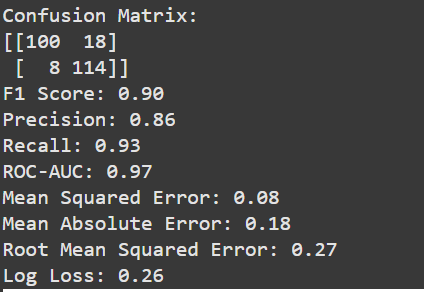
\includegraphics[width=0.85\linewidth]{evaluation-metrics.PNG}
    \caption{Evalutation Metrics}
\end{figure}
\section {Key Observations} 
\begin{itemize}
    \item The system successfully detects stampede risks with high accuracy across different crowd densities. The ROC-AUC score of 0.97 indicates that the model is highly effective at distinguishing between high-risk and low-risk stampede situations. This demonstrates strong classification capability, reducing misclassification errors.
    \item Model has high detection rates in dimly lit environments, ensuring functionality in nighttime or indoor settings.
    \item The F1 Score of 0.96 reflects a well-balanced model that maintains both high precision (0.86) and high recall (0.93).
    \item The high recall ensures that the system effectively identifies most stampede risks, minimizing the chances of missing dangerous situations.
    \item The good precision indicates that false positives are well controlled, preventing unnecessary alerts enhancing reliability.
    \item Mean Squared Error (MSE) of 0.08, MAE of 0.18, and RMSE of 0.27 signify that the model's predictions closely align with actual values, highlighting its robustness in estimating crowd density and risk levels.
    \item The low log loss (0.26) further supports the reliability of probability-based predictions, ensuring that the confidence scores assigned to different classifications are well-calibrated.
    \item The system performs well on various datasets, including JHU-CROWD++, ShanghaiTech.
\end{itemize}

\chapter{Conclusion}
The hybrid model for stampede detection and analysis using YOLOv5, Mask R-CNN and Time-Series Transformer has passed all key tests, ensuring that individual modules, integrated components, and the full system function correctly. The system achieves high accuracy with minimal errors, successfully detecting stampede risks across varying crowd densities. Its strong balance between precision and recall, along with low error rates, ensures both reliability and efficiency. The final accuracy achieved in classification is 89\%, demonstrating strong model performance.


\chapter{Appendix A : Glossary}

\begin{itemize}
    \item \textbf{ML}: Machine Learning, the study of algorithms and statistical models that computer systems use to perform tasks without explicit instructions.
    \item \textbf{DL}: Deep Learning, a subset of machine learning that uses neural networks with many layers (depth).
    \item \textbf{CNN}: Convolutional Neural Network, a deep learning algorithm used for image recognition and classification.
    \item \textbf{RCNN}: Region-based Convolutional Neural Network, an object detection model that uses selective search to extract regions of interest.
    \item \textbf{Faster R-CNN} :An improved version of R-CNN that uses a Region Proposal Network (RPN) to enhance speed and accuracy in object detection.
    \item \textbf{Mask R-CNN} : An extension of Faster R-CNN that adds a segmentation branch, allowing it to classify objects and generate pixel-level masks.
    \item \textbf{YOLO (You Only Look Once)} : A real-time object detection algorithm that predicts bounding boxes and class probabilities in a single forward pass.
    \item \textbf{Transformer} : A deep learning architecture based on self-attention mechanisms, widely used in natural language processing (NLP) and computer vision.
    \item \textbf{ViT (Vision Transformer): } : A deep learning model that applies Transformer architectures to images by dividing them into patches, achieving high accuracy in image classification tasks.
    \item \textbf{CCTV}: Closed-Circuit Television, a video surveillance system.
    \item \textbf{FPS}: Frames Per Second, a measure of how many images (frames) are captured or displayed per second.
    \item \textbf{RPN}: Region Proposal Network, part of RCNN, used for proposing candidate regions in an image for object detection.
    \item \textbf{HCI}: Human-Computer Interaction, the study of the interaction between people (users) and computers.
    \item \textbf{MII}: Motion Information Image, used to represent the movement in a sequence of images for crowd behavior analysis.
    \item \textbf{Gradio:} Enables an interactive web-based interface for real-time object detection.
    \item \textbf{PIL (Pillow):} Used for image loading and manipulation.
    \item \textbf{Argparse:} Used for command-line  argument parsing to configure model parameters.
    \item \textbf{Non-Maximum Suppression (NMS) :} A post-processing technique used in object detection to remove redundant bounding boxes by keeping only the one with the highest confidence score while suppressing others that overlap significantly.
    \item \textbf{UI}: User Interface, the space where interactions between humans and machines occur.
    \item \textbf{GUI}: Graphical User Interface, a type of user interface that allows users to interact with electronic devices using graphical icons.
    \item \textbf{API}: Application Programming Interface, a set of tools and definitions for building application software.
    \item \textbf{System:} A composite of equipment, skills, and techniques capable of performing or supporting an operational role or both. A complete system includes all equipment, related facilities, materials, software, services, and personnel required for its operation and support to the degree that it can be considered a self-sufficient item in its intended operational environment.
\end{itemize}

\chapter{Appendix B : Acronyms}
  \begin{itemize}
        \item ML: Machine Learning
        \item DL: Deep Learning
        \item LSTM: Long Short-Term Memory
        \item CNN: Convolutional Neural Network
        \item RCNN: Region-based Convolutional Neural Network
        \item RPN: Region Proposal Network  
        \item ViT: Vision Transformer  
        \item PVT: Pyramid Vision Transformer  
        \item YOLO: You Only Look Once  
        \item M-CNN:  Multi-Column Convolutional Neural Network 
        \item KNN: K-Nearest Neighbour 
        \item SVM: Support Vector Machine 
        \item ReLU: Rectified Linear Unit  
        \item IDE: Integrated Development Environment 
        \item OpenCV: Open Computer Vision 
        \item OS: Operating System 
        \item CP-CNN: Contextual Pyramid Convolutional Neural Networks
        \item CSV: Comma-Separated Values  
        \item NMS: Non-Maximum Suppression  
        \item CCTV: Closed-Circuit Television  
        \item FPS: Frames Per Second  
        \item HCI: Human-Computer Interaction  
        \item GIT: Global Information Tracker  
        \item API: Application Programming Interface  
        \item UI: User Interface  
        \item GUI: Graphical User Interface  
\end{itemize}
 
\chapter{Future Scope}
The \textbf{A Hybrid Model for Stampede Detection and Analysis Using YOLOv5, Mask R-CNN, and Time-Series Transformer} has the potential for significant enhancements in future iterations. By incorporating advanced machine learning techniques and integrating multi-modal data sources, the system can improve its predictive capabilities and situational awareness. Additionally, scalability for various event sizes and the integration of aerial surveillance could further enhance crowd management strategies.

\begin{itemize}
    \item Incorporation of multi-modal data sources, such as social media and mobile applications, for real-time crowd sentiment analysis.
    \item Development of scalable solutions adaptable to different event sizes, from small gatherings to large festivals.
    \item Implementation of drone technology for aerial surveillance and rapid assessment of crowd conditions.
\end{itemize}

\begin{thebibliography}{999}
\addcontentsline{toc}{chapter}{Bibliography}

    \bibitem{kamra2024}
    V. Kamra, A. Vaishnav, A. Verma, R. Khan, and S. Singh, "A Novel Approach for Crowd Analysis and Density Estimation by Using Machine Learning Techniques," 2024 International Conference on Intelligent Systems for Cybersecurity (ISCS), Gurugram, India, 2024, pp. 1-6, doi: 10.1109/ISCS61804.2024.10581174.
    
    \bibitem{alajlan2020}
    A. Alajlan, A. Edris, F. Sheldon, and T. Soule, "Machine Learning for Dense Crowd Direction Prediction Using Long Short-Term Memory," 2020 International Conference on Computational Science and Computational Intelligence (CSCI), Las Vegas, NV, USA, 2020, pp. 686-689, doi: 10.1109/CSCI51800.2020.00125.
    
    \bibitem{liang2022}
    D. Liang, X. Chen, W. Xu, et al., "TransCrowd: weakly-supervised crowd counting with transformers," \textit{Sci. China Inf. Sci.}, vol. 65, no. 160104, 2022, doi: 10.1007/s11432-021-3445-y.
    \bibitem{crowdformer}
    Yang, Shaopeng and Guo, Weiyu and Ren, Yuheng, "CrowdFormer: An Overlap Patching Vision Transformer for Top-Down Crowd Counting",  Proceedings of the Thirty-First International Joint Conference on Artificial Intelligence, {IJCAI-22} International Joint Conferences on Artificial Intelligence Organization, Lud De Raedt,1545--1551,7, 2022, doi : 10.24963/ijcai.2022/215.

    \bibitem{kalsotra2021}
    Rudrika Kalsotra and Sakshi Arora. 2021, "Background subtraction for moving object detection: explorations of recent developments and challenges", Vis. Comput. 38, 12 (Dec 2022), 4151–4178, doi : 10.1007/s00371-021-02286-0.

    \bibitem{garcia2020}
    Belmar Garcia-Garcia, Thierry Bouwmans, Alberto Jorge Rosales Silva, "Background subtraction in real applications: Challenges, current models and future directions", Computer Science Review, Volume 35, 2020, 100204, ISSN 1574-0137,doi: 10.116/j.cosrev.2019.100204.
    
    \bibitem{wong2023}
    V. W. H. Wong and K. H. Law, "Fusion of CCTV Video and Spatial Information for Automated Crowd Congestion Monitoring in Public Urban Spaces," \textit{Algorithms}, vol. 16, no. 3, p. 154, 2023, doi: 10.3390/a16030154.
    
    \bibitem{cob2021}
    A. C. Cob-Parro, C. Losada-Gutiérrez, M. Marrón-Romera, A. Gardel-Vicente, I. Bravo-Muñoz, and M. I. Sarker, "A proposal on stampede detection in real environments," in \textit{2021 International Conference on Indoor Positioning and Indoor Navigation (IPIN 2021)}, Lloret de Mar, Spain, Dec. 2021, pp. 1-10, ISBN: 978-1-6654-0402-0.

    
    \bibitem{fu2018}
    J. Fu, H. Yang, P. Liu, and Y. Hu, "A CNN-RNN Neural Network Join Long Short-Term Memory For Crowd Counting and Density Estimation," 2018 IEEE International Conference on Advanced Manufacturing (ICAM), Yunlin, Taiwan, 2018, pp. 471-474, doi: 10.1109/AMCON.2018.8614939.

    \bibitem{vit2021}L. Yuan et al., "Tokens-to-Token ViT: Training Vision Transformers from Scratch on ImageNet," 2021 IEEE/CVF International Conference on Computer Vision (ICCV), Montreal, QC, Canada, 2021, pp. 538-547, doi: 10.1109/ICCV48922.2021.00060. 

    \bibitem{wang2021pvt}
    Wenhai Wang, Enze Xie, Xiang Li, Deng-Ping Fan, Kaitao Song, Ding Liang, Tong Lu, Ping Luo, and Ling Shao. "Pyramid vision transformer: A versatile backbone for dense prediction without convolutions", arXiv preprint arXiv:2102.12122, 2021

    \bibitem{attention}
      shish Vaswani and Noam Shazeer and Niki Parmar and Jakob Uszkoreit and Llion Jones and Aidan N. Gomez and Lukasz Kaiser and Illia Polosukhin, "Attention Is All You Need", 2023, arXiv archivePrefix:1706.03762.
    
    \bibitem{sindagi2022}
    V. A. Sindagi, R. Yasarla, and V. M. Patel, "JHU-CROWD++: Large-Scale Crowd Counting Dataset and A Benchmark Method," \textit{IEEE Transactions on Pattern Analysis and Machine Intelligence}, vol. 44, no. 5, pp. 2594-2609, May 2022, doi: 10.1109/TPAMI.2020.3035969.

    \bibitem{wen2023transformerstimeseriessurvey}
      Qingsong Wen and Tian Zhou and Chaoli Zhang and Weiqi Chen and Ziqing Ma and Junchi Yan and Liang Sun, "Transformers in Time Series: A Survey", 2023, arXiv archivePrefix: 2202.07125.

    \bibitem{cvt}
    H. Wu et al., "CvT: Introducing Convolutions to Vision Transformers," 2021 IEEE/CVF International Conference on Computer Vision (ICCV), Montreal, QC, Canada, 2021, pp. 22-31, doi: 10.1109/ICCV48922.2021.00009. 
    
    \bibitem{parmar2018}
    Niki Parmar, Ashish Vaswani, Jakob Uszkoreit, Lukasz Kaiser, Noam Shazeer, Alexander Ku, and Dustin Tran. "Image transformer", In International Conference on Machine Learning, pages 4055–4064. PMLR, 2018.

    \bibitem{jung2022} 
    Hyun-Ki Jung and Gi-Sang Choi, "Improved YOLOv5: Efficient Object Detection Using Drone Images", 2022.
    
    \bibitem{catsanddogs}
    Omkar M. Parkhi, Andrea Vedaldi, Andrew Zisserman, and C. V. Jawahar, "Cats and dogs", In IEEE Conference on Computer Vision and Pattern Recognition, 2012.

    \bibitem{hu2019}
    Han Hu, Zheng Zhang, Zhenda Xie, and Stephen Lin, "Local relation networks for image recognition", arXiv preprintarXiv: 1904.11491, 2019. 

    \bibitem{direkoglu2020}
    C. Direkoglu, "Abnormal Crowd Behavior Detection Using Motion Information Images and Convolutional Neural Networks," \textit{IEEE Access}, vol. 8, pp. 80408-80416, 2020, doi: 10.1109/ACCESS.2020.2990355.

    \bibitem{python_docs}
    Python Documentation. [Online]. Available: \url{docs.python.org/3/}. [Accessed: September. 9, 2024].
    
    \bibitem{re9} www.stackoverflow.com

\end{thebibliography}
\end{document}
